% Institute of Computer Science thesis template
% authors: Sven Laur, Liina Kamm
% last change Tõnu Tamme 03.05.2019
%--
% Compilation instructions:
% 1. Choose main language on line 55-56 (English or Estonian)
% 2. Compile 1-3 times to get refences right
% pdflatex bachelors-thesis-template
% bibtex bachelors-thesis-template
%--
% Please use references like this:
% <text> <non-breaking-space> <cite/ref-command> <punctuation>
% This is an example~\cite{example}.

\documentclass[12pt]{article}

% A package for setting layout and margins for your thesis 
\usepackage[a4paper]{geometry}

%%=== A4 page setup ===
%\setlength{\paperwidth}{21.0cm} 
%\setlength{\paperheight}{29.7cm}
%\setlength{\textwidth}{16cm}
%\setlength{\textheight}{25cm}


% When you write in Estonian then you want to use text with right character set
% By default LaTeX does not know what to do with õäöu letters. You have to specify
% a correct input and font encoding. For that you have to Google the Web     
%
% For TexShop under MacOS X. The right lines are 
%\usepackage[applemac]{inputenc}
%\usepackage[T1]{fontenc} %Absolutely critical for *hyphenation* of words with non-ASCII letters.
%
% For Windows and Linux the right magic lines are   
% \usepackage[latin1]{inputenc}
% \usepackage[latin5]{inputenc}
%
\usepackage[utf8]{inputenc} %standard encoding since 2018 (can be commented out?)
\usepackage[T1]{fontenc} %Absolutely critical for *hyphenation* of words with non-ASCII letters.

% Typeset text in Times Roman instead of Computer Modern (EC)
\usepackage{times}

% Suggested packages:
\usepackage{microtype}  %towards typographic perfection...
\usepackage{inconsolata} %nicer font for code listings. (Use \ttfamily for lstinline bastype)


% Use package babel for English or Estonian 
% If you use Estonian make sure that Estonian hyphenation is installed 
% - hypen-estonian or eehyp packages
%
%===Choose the main language in thesis
\usepackage[estonian, english]{babel} %the thesis is in English 
%\usepackage[english, estonian]{babel} %the thesis is in Estonian


% Change Babel document elements 
\addto\captionsestonian{%
  \renewcommand{\refname}{Viidatud kirjandus}%
  \renewcommand{\appendixname}{Lisad}%
}


% If you have problems with Estonian keywords in the bibliography
\usepackage[backend=biber,sorting=none]{biblatex}
%\usepackage[style=alphabetic]{biblatex}
%% plain --> \usepackage[style=numeric]{biblatex}
%% abbrv --> \usepackage[style=numeric,firstinits=true]{biblatex}
%% unsrt --> \usepackage[style=numeric,sorting=none]{biblatex}
%% alpha --> \usepackage[style=alphabetic]{biblatex}
%\DefineBibliographyStrings{estonian}{and={ja}}
\addbibresource{references.bib}


% General packages for math in general, theorems and symbols 
% Read ftp://ftp.ams.org/ams/doc/amsmath/short-math-guide.pdf for further information
\usepackage{amsmath} 
\usepackage{amsthm}
\usepackage{amssymb}

% Optional calligraphic fonts    
% \usepackage[mathscr]{eucal}

% Print a dot instead of colon in table or figure captions
\usepackage[labelsep=period]{caption}

% Packages for building tables and tabulars 
\usepackage{array}
\usepackage{tabu}   % Wide lines in tables
\usepackage{xspace} % Non-eatable spaces in macros

% Including graphical images and setting the figure directory
\usepackage{graphicx}
\graphicspath{{figures/}}
\usepackage[section]{placeins}

% Packages for getting clickable links in PDF file
%\usepackage{hyperref}
\usepackage[hidelinks]{hyperref} %hide red (blue,green) boxes around links
\usepackage[all]{hypcap}


% Packages for defining colourful text together with some colours
\usepackage{color}
\usepackage{xcolor} 
%\definecolor{dkgreen}{rgb}{0,0.6,0}
%\definecolor{gray}{rgb}{0.5,0.5,0.5}
\definecolor{mauve}{rgb}{0.58,0,0.82}


% Standard package for drawing algorithms
% Since the thesis in article format we must define \chapter for
% the package algorithm2e (otherwise obscure errors occur) 
\let\chapter\section
\usepackage[ruled, vlined, linesnumbered]{algorithm2e}

% Fix a  set of keywords which you use inside algorithms
\SetKw{True}{true}
\SetKw{False}{false}
\SetKwData{typeInt}{Int}
\SetKwData{typeRat}{Rat}
\SetKwData{Defined}{Defined}
\SetKwFunction{parseStatement}{parseStatement}


% Nice todo notes
\usepackage{todonotes}

% comments and verbatim text (code)
\usepackage{verbatim}


% Proper way to create coloured code listings
\usepackage{listings}
\lstset{ 
  %language=python,                % the language of the code
  language=C++,
  basicstyle=\footnotesize,        % the size of the fonts that are used for the code
  %numbers=left,                   % where to put the line-numbers
  %numberstyle=\footnotesize,      % the size of the fonts that are used for the line-numbers
  numberstyle=\tiny\color{gray}, 
  stepnumber=1,                    % the step between two line-numbers. If it's 1, each line 
                                   % will be numbered
  numbersep=5pt,                   % how far the line-numbers are from the code
  backgroundcolor=\color{white},   % choose the background color. You must add \usepackage{color}
  showspaces=false,                % show spaces adding particular underscores
  showstringspaces=false,          % underline spaces within strings
  showtabs=false,                  % show tabs within strings adding particular underscores
  frame = lines,
  %frame=single,                   % adds a frame around the code
  rulecolor=\color{black},		   % if not set, the frame-color may be changed on line-breaks within 
                                   % not-black text (e.g. commens (green here))
  tabsize=2,                       % sets default tabsize to 2 spaces
  captionpos=b,                    % sets the caption-position to bottom
  breaklines=true,                 % sets automatic line breaking
  breakatwhitespace=false,         % sets if automatic breaks should only happen at whitespace
  %title=\lstname,                 % show the filename of files included with \lstinputlisting;
                                   % also try caption instead of title
  keywordstyle=\color{blue},       % keyword style
  commentstyle=\color{dkgreen},    % comment style
  stringstyle=\color{mauve},       % string literal style
  escapeinside={\%*}{*)},          % if you want to add a comment within your code
  morekeywords={*,game, fun}       % if you want to add more keywords to the set
}


% Obscure packages to write logic formulae and program semantics
% Unless you do a bachelor thesis on program semantics or static code analysis you do not need that
% http://logicmatters.net/resources/ndexamples/proofsty3.html <= writing type rules => use semantic::inference
% ftp://tug.ctan.org/tex-archive/macros/latex/contrib/semantic/semantic.pdf
\usepackage{proof}
\usepackage{semantic} 
\setlength{\inferLineSkip}{4pt}
\def\predicatebegin #1\predicateend{$\Gamma \vdash #1$}

% If you really want to draw figures in LaTeX use packages tikz or pstricks
% However, getting a corresponding illustrations is really painful  


% Define your favorite macros that you use inside the thesis 
% Name followed by non-removable space
\newcommand{\proveit}{ProveIt\xspace}

% Macros that make sure that the math mode is set
\newcommand{\typeF}[1] {\ensuremath{\mathsf{type_{#1}}}\xspace}
\newcommand{\opDiv}{\ensuremath{\backslash \mathsf{div}}\xspace} 

% Nice Todo box
\newcommand{\TODO}{\todo[inline]}

% A way to define theorems and lemmata
\newtheorem{theorem}{Theorem}

\setlength{\parskip}{2mm}

%%% BEGIN DOCUMENT
\begin{document}

%===BEGIN TITLE PAGE
\thispagestyle{empty}
\begin{center}

\iflanguage{english}{%
\large
UNIVERSITY OF TARTU\\%[2mm]
Institute of Computer Science\\
Software Engineering Curriculum\\%[2mm]
}{%
TARTU ÜLIKOOL\\
Arvutiteaduse instituut\\
Informaatika õppekava\\%[2mm]
}%\iflanguage

%\vspace*{\stretch{5}}
\vspace{25mm}

\Large Mustafa Ogün Öztürk

\vspace{4mm}

\huge Evaluating Maintainability of Android Applications: Mooncascade Case Study 

%\vspace*{\stretch{7}}
\vspace{20mm}

\iflanguage{english}{%
\Large Master's Thesis (30 ECTS)
}{%
\Large Magistritöö (30 EAP)
}%\iflanguage

\end{center}

\vspace{2mm}

\begin{flushright}
 {
 \setlength{\extrarowheight}{5pt}
 \begin{tabular}{r l} 
  \sffamily \iflanguage{english}{Supervisor}{Juhendaja}: & \sffamily Jakob Mass, MSc \\
 \end{tabular}
 }
\end{flushright}

%\vspace*{\stretch{3}}
%\vspace{10mm}

\vfill
\centerline{Tartu 2021}

%===END TITLE PAGE

% If the thesis is printed on both sides of the page then 
% the second page must be must be empty. Comment this out
% if you print only to one side of the page comment this out
%\newpage
%\thispagestyle{empty}    
%\phantom{Text to fill the page}
% END OF EXTRA PAGE WITHOUT NUMBER


%===COMPULSORY INFO PAGE
\newpage
%=== Info in English
\newcommand\EngInfo{{%
\selectlanguage{english}
\noindent\textbf{\large Evaluating Maintainability of Android Applications: Mooncascade Case Study}

\vspace*{3ex}

\noindent\textbf{Abstract:}

\noindent
%\textsc{Whitespace}
Android became one of the most comprehensive mobile platforms in the last decade.  This comprehensiveness also brought more challenges to the Android application development. Android’s nature, demanding business needs, the frequent update rate of Android applications, and lastly, changing development teams are the four major challenges for Android applications. Maintainability is defined as how easy it is to update, modify, and maintain software. At this point, maintainability emerges as a key concept because developing maintainable Android applications facilitate the above-mentioned difficulties. The primary goal of this study is to evaluate the impact of the technologies and the methods used to develop Android applications by Mooncascede, a software product development company, on maintainability. These methods and technologies include principles (e.g. Clean Code, SOLID), architectural/design patterns (Clean Architecture, MVVM), and third-party libraries (RxJava, Dagger 2 and so on). The evaluation was conducted using the triangulation strategy, which is a mixed-method approach. Qualitative evaluation was conducted via interviews with the case company's Android team (7 participants) and an Android developer survey filled by anonymous developers (over 150 participants). Also, quantitative evaluation was made via object-oriented software metrics. Study results reveal the positive impact of the evaluated methods and technologies on the maintainability of Android applications while pointing to the need for improvements. Results also indicate the need for a new maintainability model specific to the Android applications.

\vspace*{1ex}

\noindent\textbf{Keywords:} Android, Maintainability, Object-Oriented Metrics, Software Engineering

\vspace*{1ex}

\noindent\textbf{CERCS:} P170 Computer science, numerical analysis, systems, control

\vspace*{1ex}
}}%\newcommand\EngInfo


%=== Info in Estonian

\newcommand\EstInfo{{%
\selectlanguage{estonian}
\newpage
\noindent\textbf{\large Androidi rakenduste hooldatavuse hindamine: Mooncascade juhtumianalüüs}
\vspace*{1ex}

\noindent\textbf{Lühikokkuvõte:} 

\noindent
Android on saanud viimase kümnendi üheks kõikehõlmavaimaks mobiiliplatvormiks.  Samas on see omadus toonud kaasa ka katsumusi Androidi rakenduste arendamisel. Androidi rakenduste puhul on neli peamist proovikivi Androidi olemus, nõudlikud ärivajadused, rakenduste sagedane uuendamine ja muutuvad arendusmeeskonnad. Hooldatavus tähistab seda, kui lihtne on tarkvara uuendada, muuta ja hooldada. Praegu on sellest kujunemas peamine parameeter, sest hooldatavate Androidi rakenduste arendamine leevendab eelmainitud probleeme. Uurimuse põhieesmärk on hinnata Androidi rakenduste arendamisel tarvaarendusettevõtte Mooncascade kasutatud tehnoloogia ja meetodite mõju hooldatavusele. Need meetodid ja tehnoloogia hõlmavad põhimõtteid (nt Clean Code ehk puhas kood, SOLID), arhitektuurilisi ja disainimustreid (Clean Architecture ehk puhas arhitektuur, MVVM) ning kolmandate poolte teeke (RxJava, Dagger 2 jne). Hindamisel kasutati mitut meetodit hõlmavat triangulatsioonistrateegiat. Kvalitatiivse hindamise käigus tehti intervjuud uuritava ettevõtte Androidi meeskonnaga (7 osalejat) ja korraldati anonüümne küsimustik Androidi arendajatele (üle 150 osaleja). Lisaks tehti objektorienteeritud tarkvara näitajate kvantitatiivne hindamine. Uurimuse tulemustest nähtub hinnatud meetodite ja tehnoloogia positiivne mõju Androidi rakenduste hooldatavusele, aga ka täiustusvajadus. Samuti selgus tulemustest vajadus uue hooldatavusmudeli järele, mis on spetsiifiline Androidi rakendustele.

\vspace*{1ex}

\noindent\textbf{Võtmesõnad:} Android, hooldatavus, objektile suunatud mõõdikud, tarkvaratehnika

\vspace*{1ex}

\noindent\textbf{CERCS:} P170 Arvutiteadus, arvanalüüs, süsteemid, kontroll

\vspace*{1ex}
}}%\newcommand\EstInfo

%=== Determine the order of languages on Info page
\iflanguage{english}{\EngInfo}{\EstInfo}
\iflanguage{estonian}{\EngInfo}{\EstInfo}

\newpage
\tableofcontents

% Remember to remove this from the final thesis version
\newpage
\listoftodos[Unsolved issues]
% END OF TODO PAGE 

\newpage
\section{Introduction}
\label{section:1}
In the last decade, the impact of smartphones on our lives has significantly increased, and smartphones and mobile applications became people's primary way of interacting with technology. This situation has made the applications that work on these smartphones a vital part of daily and business life, from ordinary people to large companies. Today, mobile applications have become one of the most critical parts of digitalisation. Notably, as a successful open-source mobile operating system, Android has been a core element of this change, and the demand for Android applications has increased. Android application development has become one of the most necessary parts of the business area with a significant market share. Today, there are more than 2.5 billion active Android devices in the world \cite{1} . Therefore, it is difficult to ignore the importance of Android application development.
However, the increasing importance of the mobile era also brought more challenges to mobile application development and, of course, to Android application development.

Mooncascade is a  product development company based in Estonia. The company provides different software development services to its clients, including Android development. With the increasing demand for the mobile applications, the company has been facing various challenges when providing Android application development services to different customers from different fields during the development process of Android applications. These difficulties can be examined under four major topics. Android's platform-specific complexity, sophisticated business needs, the frequent update rate of Android applications, and, lastly, growing codebases and fast-changing development teams. To overcome these challenges, "maintainability" emerges as one of the most important non-functional requirements for this purpose. Developing maintainable Android applications is the way to survive in the competitive market quickly and cost-effectively. 

This study aims to evaluate the effectiveness of the Android development methods and technologies used by Mooncascade in terms of maintainability. To that aim, both qualitative analyses (via interviews and surveys) and quantitative analysis (via object-oriented software quality metrics) are conducted. The main motivation for this study is to eliminate the problems arising from the lack of maintainability in Android application development and, thus, improve developer/team efficiency and provide time and cost efficient solutions to the clients. The target audience of this study includes Android developers and researchers who are already experienced with Android application development basics. The study only focuses on native Android application development.
 
The author contributed in understanding how Android application codebases can be measured in terms of maintainability and providing emprical data on impact of the well know Android development methods and technologies on maintainability. 

\subsection{Problem Statement}
\label{section:1.1}
Mooncascade provides software development services, including Android application development. Demand for mobile applications in the industry has been increasing in the last decade. The company has been having an increasing number of requests for Android applications and facing different challenges during the development and maintenance phases of these Android applications. These challenges are detailed as follows:

\noindent\textbf{Android platform complexity:} Android SDK is an over-engineered framework that imposes inherent complexity on the developers  \cite{56}. It is different from other software due to the application life cycle, methods for accessing resources between objects, multi-threading concept, and the layout creation process \cite{52}. An Android app consists of activities, fragments, services, broadcast receivers, and content providers provided by the Android SDK and controlled by the Android OS. The necessity of working together in harmony for all these components make Android applications complex software systems.

\noindent\textbf{Business-specific complexity:} Android applications get more and more sophisticated to fulfil increasing user needs and business requirements. Mobile applications become more functional as user and business needs increase. Consequently, the complexity of Android apps from the software development point of view increases. When this business-specific complexity comes together with the platform-specific complexity mentioned above, it will be vital to implement software engineering processes to ensure the development of high-quality Android applications \cite{2}. 

\noindent\textbf{High update rate:} Android applications have a high update rate \cite{3} because of bug fixes and the frequent addition of new features based on the changing business requirement and user needs. Thus, Android developers need to keep their applications maintainable. Because it gets harder to maintain Android applications as the codebase grows or changes \cite{34}. For that reason, Android applications should be developed in a way that modifications for new features and bug fixing can be done smoothly.

\noindent\textbf{Changing Development Teams:}  Developers of an Android application change during the life cycle of the application. Whenever a new developer joins the team, the time required to onboard a new developer to the codebase is directly related to how the Android applications are developed. Therefore, Android applications must be implemented in an orderly fashion that enables developers to quickly read and understand the app's purpose.

The team aims to develop maintainable Android applications to solve these problems and have internalized some methods and technologies for this purpose, such as coding conventions/principles (e.g. SOLID, Clean Code, Clean Architecture) and using some third-party libraries (RxJava, Dagger 2, etc.). Although these methods and technologies are widely known by the Android community and are believed to be useful for maintainability, their impact on maintainability is empirically unknown for the case company, Mooncascade. Thus, to find a suitable method for maintainability evaluation and then evaluate the impact of these tools, techniques, and technologies used by Mooncascade’s Android team in terms of maintainability, this study will answer the following research questions. 

\begin{itemize}
\item \noindent\textbf{RQ1:} What is the fitting way to evaluate the maintainability of the Android applications developed by Mooncascade?
\item \noindent\textbf{RQ2:} What is the impact of the methods and technologies used by Mooncascade to develop Android applications on the maintainability of Android applications?
\end{itemize}

To answer the first research question, research is conducted to find a suitable method for evaluating the maintainability of the Android applications. During this research, previously conducted studies in software maintainability are examined, and efforts are made to find the most suitable method for this case study. The study aimed to answer the second research question using the maintainability evaluation methods obtained from answering the first research question. For this purpose, the obtained methods are applied to two different codebases, one developed by the methods used by the case company and the other not developed by following a certain fashion.

\newpage
\section{Background}
\label{section:2}
In this section, the background related to the study topic is shared. The section covers the software engineering and Android concepts that are important for this study. Also, it covers the literature review and the way of Android development at Mooncascade. Thus, to facilitate the understanding of maintainability, which is the focal point of this study.

\subsection{Android Platform}
Android is an open-source operating system for mobile devices. The Android project/operating system was initially created by the Open Handset Alliance which includes organizations from various industries such as Google, Vodafone, T-Mobile, LG, Huawei, Asus, Acer, and eBay to give some examples \cite{6}. To be more specific, Android is an open-source software stack made for a varied range of mobile devices with different structure parameters. The main goal of the Android project is to provide an open software platform accessible for a variety of stakeholders such as developers, engineers, carriers, and device manufacturers to turn their innovative and imaginative ideas into successful real-world products that improve the mobile experience for the end-users. Today, numerous organizations from Open Handset Alliance and also other organizations are supporting and investing in Android and the project is led by Google. Android is designed in a distributed way to avoid the issue of the central point of failure. In another means, different industry players confine or control the advancements of another. As a result, a production-quality consumer product comes along with open source code that is ready for customization \cite{5}.

The platform architecture of Android consists of 6 major layers. Each layer has its own responsibility and handles a different area of the Android operating system. The following figure demonstrates the layers in a way that they are ordered from the highest level of abstraction from the top to the bottom.
\begin{figure}
    \centering
    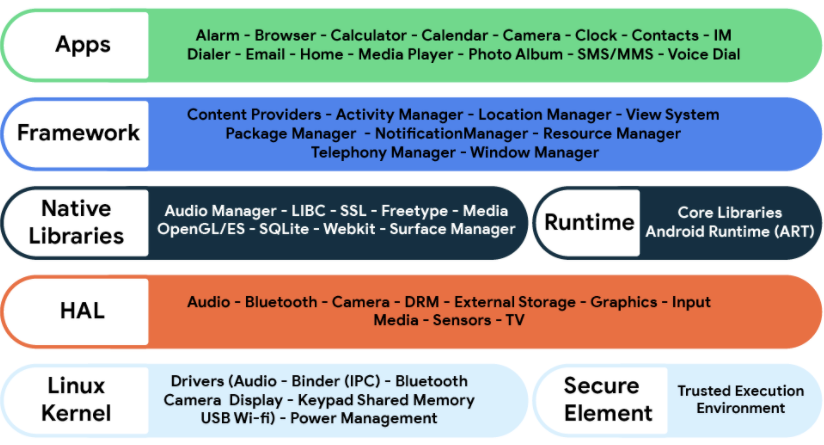
\includegraphics[scale=0.5]{figures/android_os.png}
    \caption{Android platform architecture \protect\cite{5}}
    \label{fig:android_platform_architecture}
\end{figure}

The section below gives a brief description of each major layer of the Android platform architecture mentioned in Fig. \ref{fig:android_platform_architecture}: 

\subsection{Key Software Engineering Concepts}
\subsubsection{Maintainability}
\textbf{\textit{"Good programmers write code that humans can understand." - Martin Fowler}} \cite{21}

A few decades ago programmers were using low-level programming languages that are working close to computer CPUs. These programming languages were designed to be understood by computers, not humans because computers lacked proper hardware, resources, and speed. Priorities back then were different. The computer programs had to be fast and less memory consuming. However, this situation has changed. Today computers are much stronger and software systems are more complex. However this situation also brought some difficulties to software development. Especially when developing large-enterprise software products, not considering how to overcome these difficulties may cause significant failures. In this context,  this new reality brought new standards to software development. New programming paradigms were born and the priorities have altered \cite{12}.

When the priorities of modern software development are analyzed today, the maintainability of software systems emerges as one of the most critical ones \cite{53}. Maintainability is how well a software system is understandable, repairable, and extendable. In other words, it is a characteristic of software that provides insights into how easily a software system can be maintained \cite{54}. Software systems are born, they live, they change, and eventually, they die. During their lifetime, new features are added, some features are removed, bugs are fixed, and often their development team changes. Usually, there is always a time gap between these changes. Developers should be able to understand the systems easily even months after. Besides, changes to the code base should be able to be done with ease without breaking the other parts of the software system. Ignoring all these might cause companies a significant amount of time and money. Developing maintainable software systems is the way to tackle such issues \cite{50}. In his famous book "Clean Code", Robert C. Martin explains how a top-rated company in the late 80s was wiped out from the business due to the lack of maintainability and poorly managed code organization \cite{11}. When the release cycles of their product extended due to the unorganized code base of their product, they were not able to fix bugs, prevent crashes, and add new features. Eventually, they had to withdraw their product from the market and went out of business. Lousy code and, consequently, lack of maintainability was the reason for this company to go out of the business. Considering the changes in software development since the 80s, this example might sound outdated. However, this real-life incident clearly shows how vital maintainability is to software systems and what fatal consequences it can cause if ignored. 

The importance of maintainability for software systems can also easily be seen when looking at its effect on the software development lifecycle and software development costs. A study has shown that the relative expense for maintaining software and dealing with its development speaks to over 90\% of its absolute expense \cite{4}. The maintenance period for a software system starts as soon as the system is developed. Thus, maintainability becomes a vital aspect for applying new customer needs, adding/removing new features, adapting to the environmental changes \cite{23}. Reports indicate that maintenance cost is 75\% of the total project cost, and the cost for maintaining source code is ten times bigger than developing the source code \cite{22}. The importance of maintainability for software systems is obvious. Also, considering the fast software development lifecycle of mobile applications, the importance of maintainability becomes even more apparent for mobile applications. Facebook's Android application is a good example of this situation\footnote{\url{https://www.apk4fun.com/history/2430/}}. In principle, mobile apps with high maintainability are easier to publish, update and provide high-quality features with less effort. That's why maintenance is considered one of the most important activities for mobile applications \cite{53}.


\subsubsection{SOLID Principles}
\label{section:SOLID}
SOLID stands for five principles \cite{26}. Following are the brief descriptions of each principle:
\begin{itemize}
    \item \textbf{The Single Responsibility Principle:} A class should have only one reason to chance.
    \item \textbf{The Open/Close Principle:} A module should be open for extension but closed for modification
    \item \textbf{The Liskov Substitution Principle:} Subclasses should be substitutable for their base classes.
    \item \textbf{The Interface Segregation Principles:} Many client specific interfaces are better than one general purpose interface 
    \item \textbf{The Dependency Inversion Principle:} Depend upon Abstractions. Do not depend upon concretions
\end{itemize}

The SOLID Design Principles are object-oriented design guidelines to satisfy software quality attributes such as understandability, modifiability, maintainability and testability. The steps to be taken to increase the maintainability of the software systems can be taken at the design stage. The SOLID Principles are very efficient when it comes to solving such design issues and increasing maintainability of software systems.  Not following SOLID principles may lead to serious maintainability problems in the software development lifecycle, such as tight coupling, code duplication, and bug fixing \cite{55}.

\subsubsection{Separation of Concerns}
Software systems have many complex concerns such as persistence, real-time constraints, concurrency, visualization, location control \cite{27}. Software engineering, first of all, aims to increase software quality, lower the expenses of software production, and assist maintenance and development \cite{28}. That is where "Separation of Concerns" (SoC) emerges as a solution. In the context of software engineering, SoC is a software design principle for separating a software system into discrete modules that each module addresses a single concern. A good application of SoC to a software system provides benefits such as increasing maintainability, reducing complexity. The borders for different concerns might differ from a software system to another. Concerns depend on the requirements of a software system and the forms of decomposition and composition. 

Android applications have different concerns such as sustain limited resource availability on mobile devices, user interface responsiveness,  interactions between application components,  network connectivity, local data storage, business domain-specific issues, frequent Android platform-level changes and so on. While dealing with these concerns developers spend a considerable amount thereby they are diverted from their main goal of building production-quality Android applications. Eliminating this complexity can be achieved through focusing on the separation of concerns and abstracting away different concerns from each other. Such a goal can be achieved by applying proper software architecture, e.g. "Clean Architecture" \cite{56}.

\subsubsection{Software Architecture}
In the Android world, the term "content provider" refers to the component that is designed to manage a mutual application data set that can be stored via a file system or a local database (e.g. SQLite) or any other kind of persistent storage. Content providers define, manage, and supply inter-application data sets. Android applications can provide content providers for other Android applications and through the content providers, any other Android application that has the necessary permissions can query the content provider to read and write data within its permissions. From the Android system perspective, a content provider can be considered as an entry point into an Android application in order to issue named data sets identified by a URI scheme. A solid example to a content provider can be given as the content provider that the Android system provides for the purpose of managing the contact information of the user between multiple apps \footnote{\url{https://developer.android.com/guide/topics/providers/content-provider-basics}}.



\subsection{Android Development at Mooncascade}
\label{section:2.3}
\textbf{\textit{"Good programmers write code that humans can understand." - Martin Fowler}} \cite{21}

In ancient times, when computers were big, heavy, and slow, programmers were limited to use low-level programming languages that are working close to computer CPUs. These were imperative programming languages, and the programs written in these programming languages were following the procedural programming paradigm. Although that approach worked fine, the biggest problem was that these programming languages were designed to be understood by computers, not humans. The main reason for this situation was that, back in that time, computers lacked proper hardware, resources, and speed. Consequently, the priorities back then were different. The computer programs had to be fast and less memory consuming. However, this situation has changed in the current day. Even a low-quality mobile device is much stronger and smarter than the computers that people were using a couple of decades ago, and software systems became complex. Although this change brought a positive impact on the end-user side as it also brought more functionality and ease, the impact it brought the software development side is complexity. Especially when developing large-enterprise software products, ignoring that fact and not considering how to overcome this complexity may cause significant failures. In this context, new programming languages and paradigms were born, the priorities have altered, and this new reality brought different challenges and new quality standards to software development \cite{12}.

When the priorities of modern software development are analyzed today, the maintainability of software systems emerges as one of the most critical priorities, perhaps even the most important. According to the IEEE Standard Glossary of Software Engineering Terminology, the term "maintainability" is the ease with which a system or component can be modified for use in applications or environments other than those for which it was specifically designed \cite{20}. In the context of software engineering, maintainability means how well a software system is understandable, repairable, and extendable. Maintenance is one of the most important parts of the software development life cycle because the time spent on maintaining software systems requires more time and resources than the rest of the process. The relative expense for maintaining software and dealing with its development speaks to over 90\% of its absolute expense \cite{4}. The level of maintainability that a software system depends on several different factors. Overall, a software system can be considered maintainable if it is simple to grasp how it works and what it does, and making changes such as adding new features and fixing bugs is easy. Besides, maintainability is directly related to well-known software engineering concepts such as coupling, complexity and cohesion. Knowing the relationship between these concepts and maintainability is also essential in measuring maintainability, which is one of the topics of this study. Previous studies have proved this relationship. The inverse ratio between complexity and maintainability was mentioned in Saifan and Rabadi (2017) on measuring maintainability in Android applications \cite{34}. Also, the inverse relationship between coupling and maintainability and the correlation between cohesion and maintainability are discussed in detail in Barak et al., (2012) on maintainability metrics in open-source software \cite{33}.

Considering the life cycle of software systems might help to understand the importance of maintainability. Software systems are born, they live, they change, and eventually, they die. However, their lifetime is generally long, and during their lifetime, new features are added, some features are removed, bugs are fixed, and often their development team changes. Usually, there is always a time gap between these changes. In other words, developers might need to make a change to the software system, which they worked in weeks or months before. In such cases, developers should be able to understand the systems easily even months after. Besides, changes to the code base should be able to be done with ease without breaking the other parts of the software system. Also, when a new developer joins the development team, onboarding should be smooth, and the new developer should be able to understand the purpose of the software system easily. Ignoring all these might cause companies a significant amount of time and money. That is what makes maintainability that important. Developing maintainable software systems is the way to tackle such issues.

The importance of maintainability for software systems can also easily be seen when looking at its role in the software development lifecycle and its effect on software development costs. The maintenance period for a software system starts as soon as the system is developed. Thus, maintainability becomes a vital aspect for applying new customer needs, adding/removing new features, adapting to the environmental changes \cite{23}. The time that has to be spent on the maintenance of complex software products is comparatively more extended than the rest of the software development lifecycle processes. Reports indicate that the amount of effort spent on software maintenance is between 65\% and 75\% of the total amount of effort \cite{13}. Also, another report points out that maintenance cost is 75\% of the total project cost, and the cost for maintaining source code is ten times bigger than developing the source code \cite{22}. In his famous book "Clean Code", Robert C. Martin explains how a top-rated company in the late 80s was wiped out from the business due to the lack of maintainability and poorly managed code organization. When the release cycles of their prominent product extended, due to the unorganized code base of their product, they were not able to fix bugs, prevent crashes, and add new features. Eventually, they had to withdraw their promising product from the market and went out of the business. Lousy code and consequently, maintainability was the reason for this company to go out of the business \cite{11}. This real-life example clearly shows how vital maintainability is to software systems and what fatal consequences it can cause if ignored.

The importance of the maintainability for software systems is evident and this situation is no different for Android Applications. In fact, the importance of maintainability for Android applications is even higher since Android applications have a very active software development life cycle. Given that the growing user demands and business needs making the Android applications more and more complex and Android applications having frequent update rates, it is not hard to see how important the maintainability is for Android application development. This situation is one of the main sources of motivation for this study. 

 In addition to that, in the context of Android, when the main challenges mentioned in this study are evaluated together, the importance of maintainability as a non-functional requirement becomes even more evident for Android application development because the high level of maintainability is the way to overcome the challenges and complexities mentioned in this study while developing Android applications. In consequence, the question is how to achieve the goal of developing Android applications with high maintainability. From the software development point of view, the Android platform does not have strict rules on how the applications are developed. Developing maintainable applications is not an obligation. However, developing Android applications with high maintainability is a need to solve the difficulties mentioned in this study in a timely and cost-efficient manner, facilitate the development processes for the Android developers, and increase the quality of the Android applications. The methods to be followed and the technologies to be used in Android applications for meeting these requirements constantly evolve, and the topic is still controversial among the Android community. Different solutions have been proposed and tried since the birth of the platform. However, the unchanged reality is that the most important criteria for building reliable software systems in a timely and cost-efficient manner is maintainability and of course, this reality is not different for Android applications. 

\subsection{Literature Review}
%\label{section:2.4}
In this chapter, the data obtained within the scope of this study about the importance of maintainability for software systems and Android applications were shared. In addition, information regarding the key concepts required to ensure the maintainability of software systems has been presented. Also, information regarding the way of Android development at Mooncascade was presented.

\subsection{Summary}
Today, the complexity of software applications is quite high, and it still is increasing. Today's software systems have many complex concerns such as persistence, real-time constraints, concurrency, visualization, location control \cite{27}. Software engineering, first of all, aims to increase software quality, lower the expenses of software production, and assist maintenance and development. In achieving these aims, software engineers are continuously on the lookout for developing technologies and approaches that increase maintainability, decrease software complexity, enhance understandability, support reuse, and boost development. That is where "Separation of Concerns" (SoC) emerges as a solution. 

In the context of software engineering, SoC is a software design principle for separating a software system into discrete modules that each module addresses a single concern. A good application of SoC to a software system provides benefits such as increasing maintainability, reducing complexity. The borders for different concerns might differ from a software system to another. Concerns depend on the requirements of a software system and the forms of decomposition and composition \cite{28}. 

In the context of Android, the importance of SoC is even more apparent. Android applications have different concerns with clearly drawn borders. Such concerns can be named as visualization and presentation of data, business logic, networking, persistence, location services. Depending on the requirements of an Android application, there might be other concerns as well. In light of the information above, it is vital to identify these concerns before Android applications are developed, and during the development phase, to use techniques that can apply SoC well.





\newpage
\addtocontents{toc}{\protect\newpage}
\section{Research Methodology}
\label{section:3}
In the first and second sections, information was given about this study's aims, the reasons for the study's emergence, and the study's motivation sources. Besides, to better understand this study's background, objectives, and solutions, the necessary information was shared with the readers in both the Android and software development fields. As stated in the previous sections, the starting point of the study is the difficulties encountered in Android application development and a non-functional requirement named maintainability, which has an important role in solving these difficulties. As stated before, this study focuses on solving these problems in Android application development and how Mooncascade, a leading software development company in the region, approaches the issue of increasing maintainability. In this context, the approaches, techniques, and technologies used by the company's Android team will be discussed, and the level of effectiveness of these will be determined in terms of maintainability. At this point, the first question that comes to mind is how this effect can be determined or measured in terms of maintainability.

In this section,  the methods to evaluate and measure how effective the techniques, technologies, and other approaches used by Mooncascade's Android team are from the maintainability perspective will be explained. These assessment and measurement methods will be both quantitative and qualitative. In this way, it was aimed to evaluate with maximum efficiency by going beyond the traditional quantitative measurement techniques. The methods to be used and the contents of these methods will be presented in detail in this section. Also, why and how these methods are chosen will be stated in this section. Thus, the first of the three research questions stated in the introduction section will be answered in this section. In the 4th section, the technologies, techniques, and approaches used by Mooncascade's Android team to increase the maintainability of Android applications and eliminate the difficulties mentioned in the previous sections will be discussed. These techniques, technologies, and approaches will be evaluated in section 5 using the measurement and evaluation techniques explained in this study. Therefore, it was thought that answering the first research question here is more appropriate before answering other research questions in the upcoming sections. The remainder of this section will provide detailed information on the quantitative and qualitative measurement techniques to be applied in this study to measure maintainability in the context of Android application development. 

\subsection{Qualitative Method}
When other academic studies dealing with the measurement of maintainability in Android or other software systems are considered, it can be seen that many studies use scientific and quantitative methods. The work of Verdecchia et al. in the maintainability and architecture of Android applications can be shown as a successful example of this situation \cite{14}. Although it cannot be claimed that such quantitative measurements are inaccurate, it would not be wrong to say that these measures are inadequate at times. It is essential to make qualitative evaluations, and quantitative evaluations in areas where technologies are rapidly developing and trends change quickly, especially in Android application development. In this way, it may be possible to measure developers' experiences that differ in the face of rapid change and development and the effects of these experiences on the maintainability issue we are working on more efficiently. For these reasons, it was deemed appropriate to add a qualitative evaluation technique to this study’s scope. An Android developer survey and some interviews were conducted within this study's scope as a part of qualitative evaluations. The contents and purposes of these surveys and conferences are discussed in detail in their respective sub-sections below.

\subsubsection{Android Developer Survey}
The first step of qualitative evaluations in this study is the Android developer survey. The consistency and stability of principles and third-party libraries used in Android applications indirectly affect the maintainability of applications. Therefore, although it does not directly contribute to measuring maintainability, this survey was conducted to identify current Android trends and provide support for this study's evaluation. While determining this survey's questions, priority was given to principles and technologies that directly and indirectly affect maintainability. Although the questions are generally prepared to cover the methods used by the Mooncascade Android's team, it can be said that the questions reflect the Android technology stack in general. The content of the survey can be accessed publicly\footnote{\url{https://forms.gle/MoiTGMV874yzJwuv8}}. The questions are organised with the help of the Forms application provided by Google. The Android developer survey has been delivered to Android developers from different companies in different countries through accounts or groups of Android developer communities on social media platforms such as LinkedIn, Discord, and Twitter. The author of the study has also shared the survey with many of his colleagues/ex-colleagues working in different companies/countries.

\subsubsection{Interviews with Team Members}
The second step of the qualitative evaluations carried out within this study’s scope is the interviews conducted with Mooncascade's Android team members. Unlike the Android developer survey that was explained in the previous section, these interviews are designed and conducted to qualitatively evaluate the techniques, technologies, and methods used by Mooncascade's Android team in terms of maintainability. Eight questions were determined to qualitatively measure the effect of the methods used by Mooncascade's Android team on the maintainability of Android applications. Below are listed the questions asked to each member of Mooncascade's Android team during these interviews:
\begin{itemize}
    \item How many years of experience do you have as an Android developer? Please specify the years in Mooncascade and other companies.
    \item How many different Android projects have you completed in Mooncascade, and how many different domains did those projects belong to?
    \item What is your understanding of maintainability in the context of software engineering?
    \item As an employee of a software development company that provides services to the different domains, what makes maintainability more essential for you?
    \item What is the importance of maintainability when developing Android applications?
    \item What is the most critical aspect for maintainability when developing Android applications (e.g. architecture, libraries, programming language, etc.)?
    \item How do you think the current technology stack of the team impacts Android applications’ maintainability? Please specify for each item below:
    \begin{itemize}
        \item Programming Languages(Kotlin/Java)
        \item Software Engineering principles (SOLID/Clean Code)
        \item Architecture (MVVM/Clean)
        \item Libraries (RxJava, Dagger 2, Apollo/Retrofit)
        \item Android Architecture Components (ViewModel, LiveData, Room, etc.)
    \end{itemize}
    \item What could be improved in our current tech stack and the principles we apply to improve the Android applications’ maintainability?
\end{itemize}

Three main criteria were taken into consideration while preparing these questions. First of all, questions were chosen to measure the participants' background, experience, and understanding of the concept of maintainability in software engineering. Subsequently, questions were drafted about technology and principles that directly or naturally affect maintainability. Finally, questions were prepared concerning the Android developer questionnaire, which was mentioned in the previous section, to make it possible to compare the results of both the survey and the interviews in the evaluation section. These questions, which are included in the interviews, were directed to the team members in the meetings conducted privately with each team member. The collected answers and information will be interpreted in detail in section \ref{section:5}. It is aimed that the knowledge and experience gathered through these interviews will support the accuracy and validity of quantitative assessments.


\subsection{Quantitative Method}
\label{section:3.2}
Quantitative evaluation constitutes the most critical part of this study in terms of measuring maintainability. As a part of this study, many other academic works on the measurement of maintainability in Android and software engineering were examined. The purpose of these reviews is to find the most appropriate maintainability measurement metrics. Various metrics can be used to evaluate object-oriented software systems in terms of quality and maintainability. The most popular of these metrics are detailed in Barak et al., (2012) \cite{33}. As a result of this examination, it was seen that the concepts of complexity, cohesion and coupling were emphasised in many studies, and it was concluded that the measurements made based on these concepts would be more efficient when measuring maintainability. The effects of these concepts on maintainability have been mentioned in the second chapter, and detailed studies in this field have been referred to. Studies have shown that results retrieved from evaluating these concepts proved to define the level of maintainability \cite{33}.

The definition of complexity in software engineering is the difficulty to understand the interactions between the parts of a software system. Higher levels of complexity in software increase the risk of accidentally preventing interactions, increasing the chance of introducing bugs when making changes, thus decreasing maintainability. High coupling between classes also causes complexity when maintaining the software. Changes done in a class reflect the dependent class due to the dependency relationship of the classes. Thus, the software system becomes challenging to maintain. In software engineering, cohesion is how well the methods of a class are related to each other. While the classes' relationship is desired to be loosely coupled, their methods and data fields are desired to be related. Lack of cohesion threatens modularity and software maintenance. 
\begin{figure}[ht!]
    \centering
    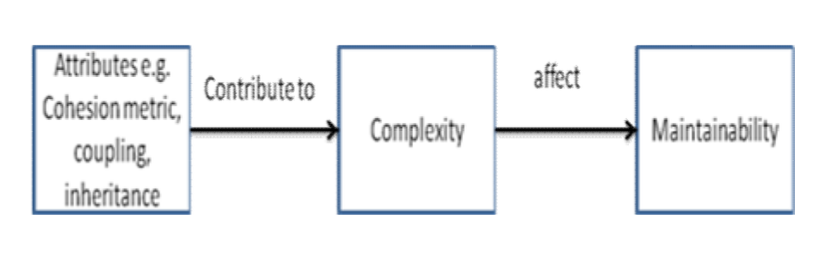
\includegraphics[scale=0.5]{figures/maintainability_factors.png}
    \caption{Relationship between cohesion, coupling, complexity and maintainability \protect\cite{33}}
    \label{fig:maintainability_factors}
\end{figure}

As can be seen, complexity, cohesion and coupling are in a tight relationship among themselves, and they all directly affect software maintainability. The figure below shows the relationship between maintainability, complexity, cohesion and coupling. Therefore, based on this result, research was done on measuring the concepts of complexity, cohesion and coupling effectively, and the most suitable metrics for measurement were determined. As a result of this research, five metrics that will enable an object-oriented software system to be evaluated effectively in terms of complexity, cohesion and coupling have been determined. While selecting these metrics, priority has been given to metrics that can handle a software system as a whole in the areas of complexity, cohesion and coupling. This enables the system to be evaluated in terms of maintainability in the most effective way. To emphasise again, although these metrics are used in measuring complexity, cohesion and coupling, they allow maintainability to be measured directly due to the tight relationship between these concepts and software maintainability. These metrics and their intended use are listed below. 
\begin{itemize}
    \item \textbf{Weighted Method Count (WMC):} This metric is used to measure object-oriented software systems’ complexity. WMC represents a class's cyclomatic complexity, also known as McCabe complexity \cite{35}. It, therefore, portrays the complexity of a class as a whole, and this measure can be used to indicate the maintainability level of the class. The number of methods and complexity can be used to divine maintaining effort. If the number of methods is high, that class is described as domain-specific and is less reusable. Also, such classes tend to be prone to change and defects.
    \item \textbf{Depth of Inheritance Tree (DIT):} This is another metric to measure software complexity. Inheritance increases software reusability; however, one side can create complexity by possibly violating encapsulation since the subclass needs to access the superclass. Furthermore, changes made during maintenance might increase the inheritance tree's depths by adding more children. Therefore, by assessing the inheritance tree available in the product, it is easy to predict how much effort needed to make it stable \cite{33}. It is harder to predict its behaviour if the tree depth is high, and this causes maintenance issues.
    \item \textbf{Number of Children (NOC):} NOC measures the number of descendants of a class, and it is used to measure the coupling level for the corresponding class. NCO also indicates the reusability level of a software system. It is assumed that the number of child classes and the maintainer's responsibility to maintain the children's behaviour are directly proportional. If the NOC level is high, it is harder to maintain and modify the class \cite{36}.
    \item \textbf{Coupling Between Object Classes (CBO):} This metric calculates the number of connections to other classes from a particular class, and it is used to measure coupling. A class is considered coupled if it depends on another class to get its work done \cite{34}. CBO metric is related to the reusability of the class. High coupling makes the code more difficult to maintain because changes in other classes can also affect that class. Therefore these classes are less reusable and less maintainable.
    \item \textbf{Lack of Cohesion of Methods (LCOM):} This metric is used to determine how class methods are related to each other, and it is applied to evaluate cohesion. Cohesion promotes the maintainability of the software systems. High cohesion for a class meant the class is understandable, maintainable and easy to modify \cite{33}.
\end{itemize}

Apart from the above metrics, many other metrics can measure quality and maintainability in object-oriented software systems. The most well-known of these metrics are the Line of Code (LOC) and Halstead Effort metrics. Studies conducted using these metrics in Android, and other software development fields were examined within this study's scope. The methods related to size were not preferred because they were too classical, and they do not give very effective results on maintainability. Halstead complexity metrics were not preferred because they concentrated more on the complexity of classes and methods. Regarding the use of these metrics, Prabowo's work on Android apps' maintainability can be examined \cite{19}. Instead, metrics that facilitate evaluating the quality and maintainability of software systems as a whole were preferred.

After determining the metrics to be used, research has been conducted on how these metrics will be applied. As a result of the research, it has been concluded that metrics can be applied manually or with a tool's help. Since manual implementation will take more time and is prone to error, it has been decided to apply metrics with a reliable tool. Later, a search was done for a static code analysis tool to work with Android Studio and Kotlin programming languages and support the selected metrics. During the research, the CodeMR static code analysis tool drew attention. CodeMR is a powerful software quality tool that is integrated with IDEs and supports multiple programming languages. Java, Scala, Kotlin and C++ \footnote{\url{https://www.codemr.co.uk}}. The tool provides an understanding of software quality through its metrics to measure coupling, complexity, cohesion and size. These metrics are often affected by various code characteristics, making them promising for evaluating software maintainability.  Besides, the tool provides a visualisation centric approach and generates detailed reports supported by different visualisation options. In this way, it facilitates the application of metrics and makes the results more understandable with detailed reports and advanced visualisation techniques. The tool can also be installed as a plugin in Android Studio and is very easy to use. Apart from that, the tool also makes it possible to measure with many other metrics. The complete list of metrics and other features that the tool offers can be accessed via the tool's documentation. Finally, 2 academic studies conducted using this tool were examined before the tool was started to be used, and information about the tool operation was obtained\cite{38}\cite{39}. Finally, the CodeMR static code analysis tool has been chosen to be used in this study due to the support of Kotlin, its ability to be installed as an add-on to Android Studio, its support for selected metrics, and its advanced visualisation and reporting mechanisms. After this decision, communication was established with the CodeMR team, and a free license was obtained to be used in academic studies. 

The use of metrics (CodeMR static code analysis tool) to measure the impact of technologies, methods and principles used by the Mooncascade Android team on maintainability was realised as described following. First of all, a pilot project where metrics can be applied has been determined. While determining the pilot project, the priority was to find a project with an old version developed using outdated technologies, methods, and a weakly structured architecture. However, this project should also have had a new version developed with current technologies and methods mentioned in this study. Thus, using the metrics mentioned above, the impact of the team's current methods on maintainability could be measured. Because of Mooncascade's wide range of realised and ongoing projects, finding a project that met these conditions was possible. Although the full content cannot be published due to the privacy principles and confidentiality, it was possible to apply quantitative evaluation by applying selected metrics to the available features of the old (actively in use) and new codebases (still under development) of an Android application. In this way, it was aimed to evaluate the effects of the methods, principles and technologies used by the Mooncascade Android team on maintainability at the maximum level effectively. Detailed information and evaluation of the results will be shared in section \ref{section:5}.

\subsection{Summary}
In this section, detailed information about the qualitative and quantitative evaluation methods performed within this study's scope was shared. The knowledge regarding these methods' contents, why they were preferred, and how they were applied were presented. Thus, the evaluation part's conduction, one of the essential parts of this study, was presented, and the first research question was answered. Detailed results of qualitative and quantitative evaluations will be shared in section \ref{section:5}.


\newpage
\section{Mooncascade Case Study}
\label{section:4}
\subsection{Case Company}

\subsection{Principles}
\subsubsection{SOLID Principles}
\label{section:4.2.1}
\subsubsection{Clean code}
\label{section:4.2.2}

\subsection{Programming Language}
\label{section:4.3}

\subsection{Architecture}
\subsubsection{MVVM}
\label{section:4.4.1}
\subsubsection{Clean Architecture}
\label{section:4.4.2}

\subsection{Libraries}


\subsubsection{Dependency Injection}
\label{section:4.5.1}
\subsubsection{Networking}
\label{section:4.5.2}
\subsubsection{Asynchronous Events}
\label{section:4.5.3}
\subsubsection{Android Architecture Components}
\label{section:4.5.4}

\subsection{Summary}

\newpage
\section{Evaluation}
\label{section:5}
In this section, the results obtained from applying quantitative and qualitative assessment methods, whose details were shared in section \ref{section:3}, will be presented. As explained in the 3rd section before, the Android developer survey findings and the results obtained from the interviews made with the Mooncascade Android team members, which were applied within the qualitative evaluation scope, will be shared in this section. The quantitative evaluations, which were detailed in the third section, will also be presented in this section. Finally, through the results obtained from the qualitative and quantitative evaluations, the third research question will also be answered in this section.

\subsection{Android Developer Survey Results}
The Android developer survey results, which is the first step of qualitative evaluations, are shared in this section. Trends have been identified regarding technologies and principles that are likely to impact the maintainability of Android applications.

\subsubsection{Conduction Period of the Survey}
The survey accepted answers between April 2020 and March 2021 and reached 164 participants in total.
\begin{figure}[ht!]
    \centering
    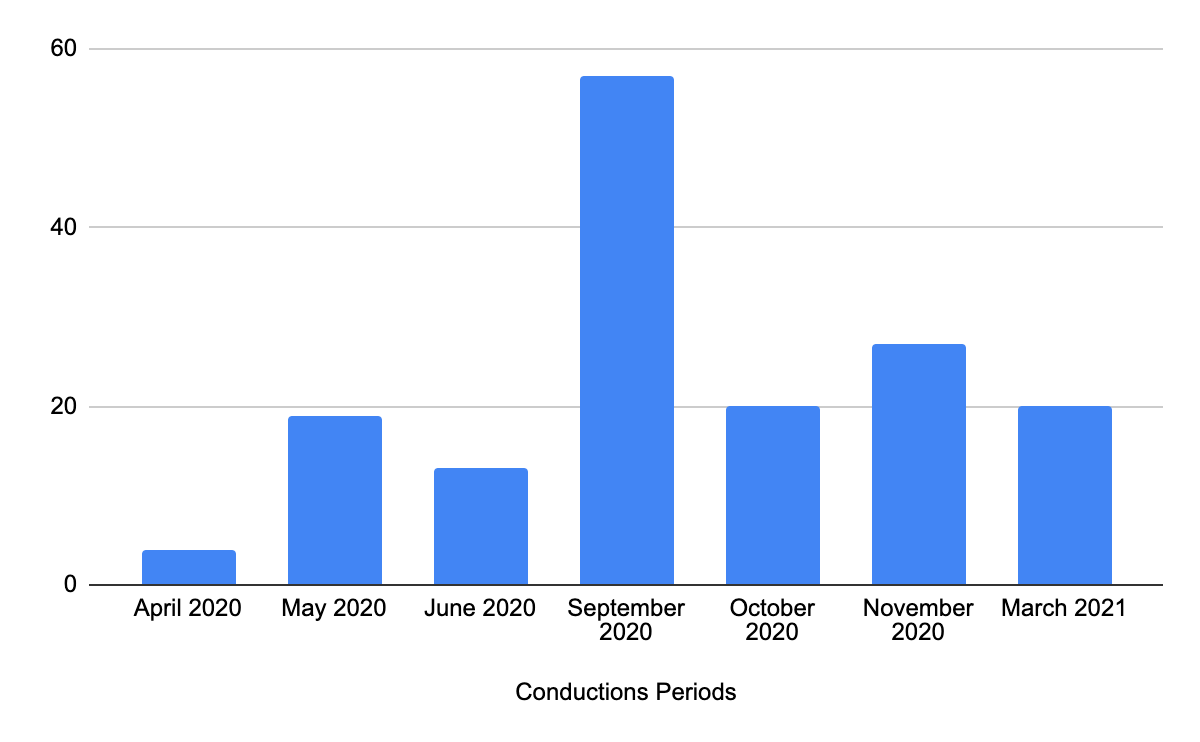
\includegraphics[scale=0.3]{figures/conduction_period.png}
    \caption{Conduction period results}
    \label{fig:conduction_period}
\end{figure}

As shown in Fig. \ref{fig:conduction_period}, participation in the survey took place only during specific periods of this one-year term. Although the questionnaire accepted answers for a year-long, it was boosted in different periods,  as shown in the histogram above. It would be logical to consider this situation while examining the response numbers.

\subsubsection{Participant Background}
In this kind of survey, it is essential to ensure the participants’ diversity to get sufficiently accurate and generally reflective results. The Android developer survey found participants through the author's current and former colleagues working in seven different well-known companies in different parts of the world. Also, as previously stated in section \ref{section:4.1.1}, the survey reached answers from random Android developers through various social media platforms. In this way, the participants’ diversity was increased, and getting more accurate results was ensured. Also, the first question was added to the survey to find out the participant competence. The experience of an Android developer impacts the developer's tendencies when making decisions such as technologies, methods, architectural pattern and so on. Responses gathered from this question can be used to identify such correlations. Results can be seen in Fig. \ref{fig:dev_experience} below.
\begin{figure}[ht!]
    \centering
    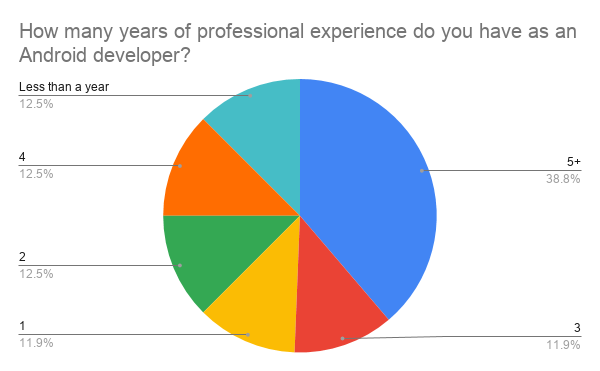
\includegraphics[scale=0.6]{figures/survey_q1_dev_experience.png}
    \caption{Participant background results}
    \label{fig:dev_experience}
\end{figure}
\FloatBarrier
When Fig. \ref{fig:dev_experience} is examined, 63\% of the participants have more than 3 years of experience while around 39\% of them has 5+ years of experience. People with 0-2 years of experience are around 37\% of the all participants.

\subsubsection{Issues}
The most severe limitation of the survey was undoubtedly in finding respondents. Even though the survey was shared on many different social media platforms and developer community pages, it was able to find very few participants compared to the number of people on these platforms and communities. The initial target for the number of participants was 150-200, and a serious effort was made to reach this number.

Besides, some corrections and filtering were made for the 164 responses collected from these Android developers to avoid off-topic responses and collect non-standard answers under a single topic, thus presenting more consistent results both visually and numerically. For some of the questions, there is the option "other" among the answer options offered, and users can choose this option and enter their answers. For example, "Toothpick" or “Hilt” libraries do not have a ready-made response option in the survey. Android developers using this library have given their answers in different forms (e.g. Toothpick and toothpick or Hilt, Dagger Hilt or hilt). Therefore, it was deemed necessary to arrange the inputs in different forms, which correspond to the same answer. 

As an example of the need to filter some answers, a situation in the chart below can be shown. As can be seen in the chart above, which was obtained from the unfiltered survey results, it is seen that developers who develop Android in other forms also participated in the survey. Although it was clearly stated to the participants that the survey covers only "Native" Android developers before they filled in the questionnaire, a few such cases were unfortunately not avoided due to the human factor. These kinds of responses have been filtered out and edited as they will not contribute to this survey’s purpose and they reduce the survey’s accuracy.
\begin{figure}[ht!]
    \centering
    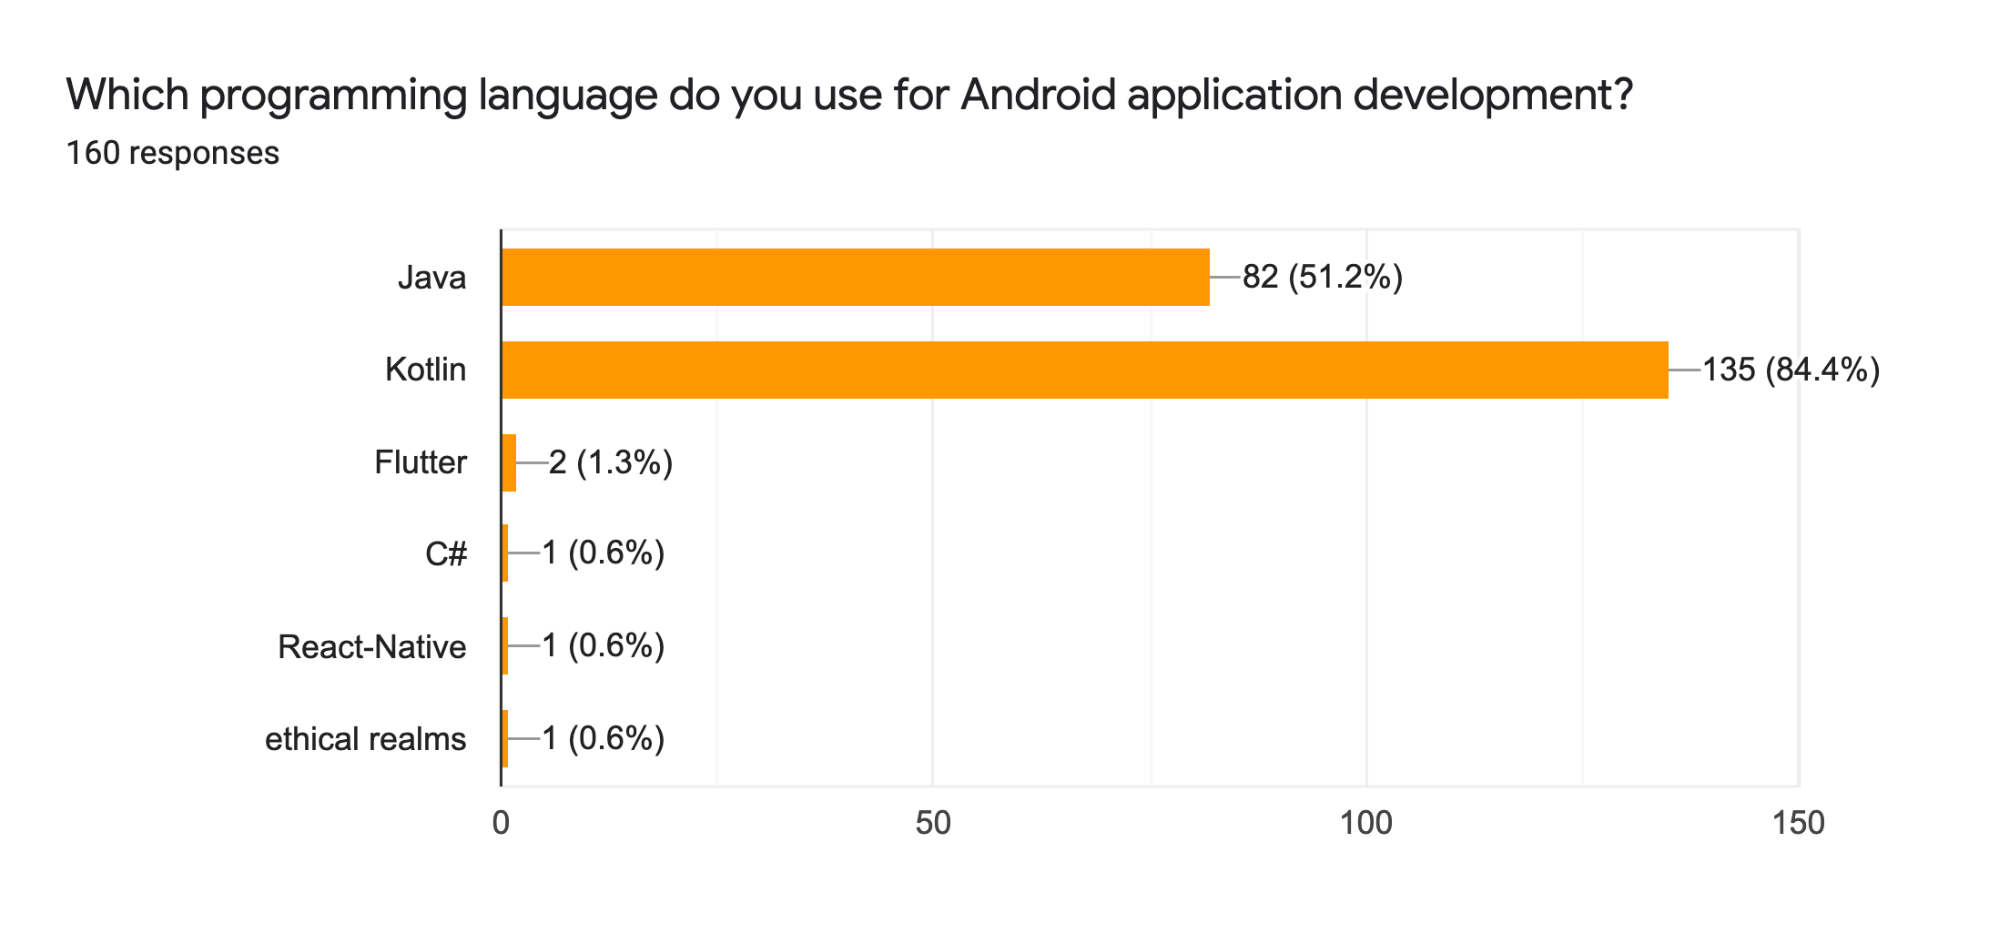
\includegraphics[scale=0.20]{figures/survey_corrupted_chart.png}
    \caption{Example chart plotted with corrupted data}
    \label{fig:corrupted_chart_example}
\end{figure}

The above and other similar situations were filtered out or edited as they will not contribute to the survey's purpose and they reduce the survey’s accuracy. Firstly, the survey results were extracted as a Google Sheets file to do this filtering and editing. Then inappropriate data in this file was corrected or filtered, and finally, the charts and numbers were obtained from the accurate data of the file. While applying corrections and filtering, no changes or manipulations were made on the relevant data. Around 20 of the 164 responses were edited to arrange the inputs in different forms, which correspond to the same answer. Besides, five corrupted responses were removed. After the filtering process, results were visualised from the filtered and updated 159 responses.  The charts obtained through filtered and corrected responses and the data obtained from these charts’ interpretation are presented below, respectively. Since it is possible to choose more than one answer for some questions, it should be taken into account that the total number of answers for each question may exceed the total number of participants.


\subsubsection{Programming Language}
The second question of the survey asks Android developers the programming language or programming languages they use to develop Android applications. As mentioned in section 2, different programming languages can be used while developing Android applications. Nevertheless, this study focuses solely on "Native" Android development, as mentioned many times before. Therefore, only Java and Kotlin programming languages are among the options offered to answer the second question.
\begin{figure}[ht!]
    \centering
    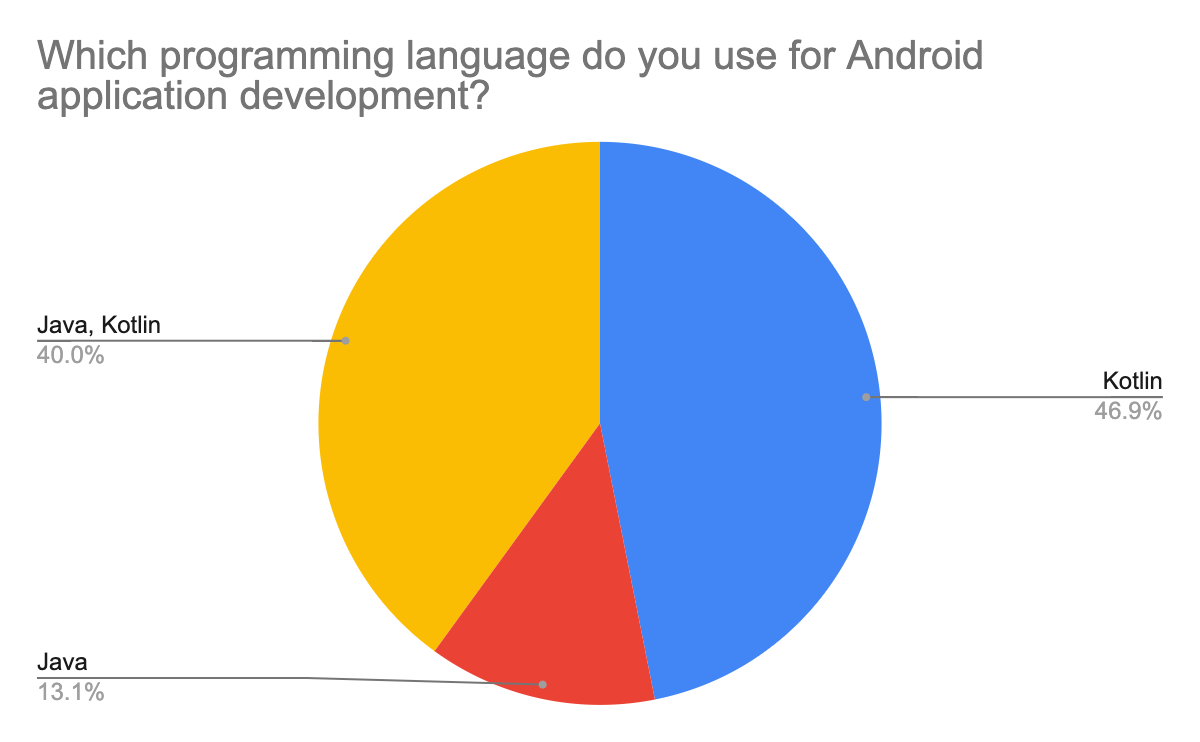
\includegraphics[scale=0.3]{figures/programming_language.png}
    \caption{Programming languages results}
    \label{fig:programming_languages}
\end{figure}

In Fig. \ref{fig:programming_languages} above, Android developers' trends regarding the programming language they use while developing "Native" Android applications can be seen. Around 47\% of the Android developers surveyed seem to use the Kotlin programming language. 40\% of the participants use Java and Kotlin together, while only 13.1\% use the Java programming language. Considering that Kotlin is a programming language suggested by Google and Android and is more "programmer-friendly" than Java, it is not difficult to understand that the above table is not surprising. As of 2020, Google declared that more than 60\% of Android applications were developed with Kotlin. It can be said that the survey results largely overlap with this statement\footnote{\url{https://developer.android.com/kotlin}}. On the other hand, he fact that some users still use Java can be explained by the existence of Android applications developed with Java before Kotlin was declared as an official programming language for Android.

As stated in section \ref{section:4.3}, Mooncascade's Android team develops Android applications using Kotlin programming language, unless otherwise requested by its customers. When the survey results presented in detail above and the company's choice are compared, it is seen that this choice coincides with the Android community’s current trends.

\subsubsection{Architecture}
The third question of the survey asks participants about their choice of presentational design patterns. In this question, MVVM, MVP, MVI, etc. design patterns were defined as presentational design patterns. When the results are  examined, a diverse set of answers were seen. Below, in Fig. \ref{fig:design_pattern} the participants' preferences for presentational design patterns are displayed.
\begin{figure}[ht!]
    \centering
    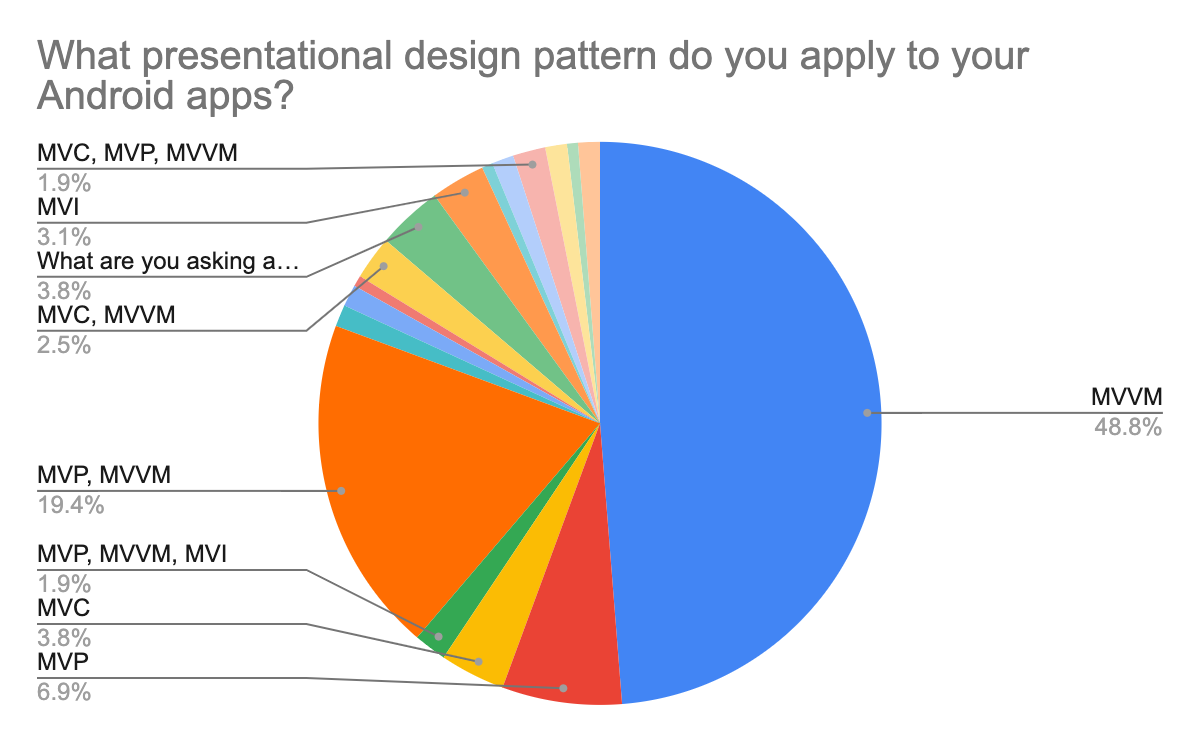
\includegraphics[scale=0.3]{figures/design_pattern.png}
    \caption{Presentational design patterns results}
    \label{fig:design_pattern}
\end{figure}
\FloatBarrier
The first notable conclusion is that almost half of the participants use the MVVM presentational design pattern. Besides, it is seen that another 25\% of the participants stated that they used this design pattern and different design patterns. In other words, a total of 3 quarters of the participants stated that they used the MVVM design pattern in some way or another. On the other hand, the chart presents us that design patterns such as MVP, MVC, MVI are also frequently used. When the participants' responses are sifted through, it is seen that design patterns such as MVP, MVC and MVI are generally preferred by some developers alongside the MVVM design pattern. These developers have more experience than those who have a single choice of design pattern. Also, it was seen that developers with 0-3 years of experience have answered this question by selecting the MVVM option. Another important detail is that 5 out of 6 participants that answered this question as "What are you asking about" had one year or less experience. Lastly, it was seen that the MVI design pattern was selected nine times in the last six months (out of 120 answers with a ratio of 0.075). However, it was selected only once (out of 40 answers with a ratio of 0.025) by the participants in the first six months in which the survey accepted answers.

In the following question, users were asked whether they use the "Clean Architecture". It is essential to mention why Clean Architecture was asked to the participants differently from the presentational design patterns. Clean Architecture allows the arrangement of an entire application in terms of architecture, unlike the presentational design patterns. The graphical breakdown of participant answers to this question is presented below in Fig \ref{fig:clean_arch}.
\begin{figure}[ht!]
    \centering
    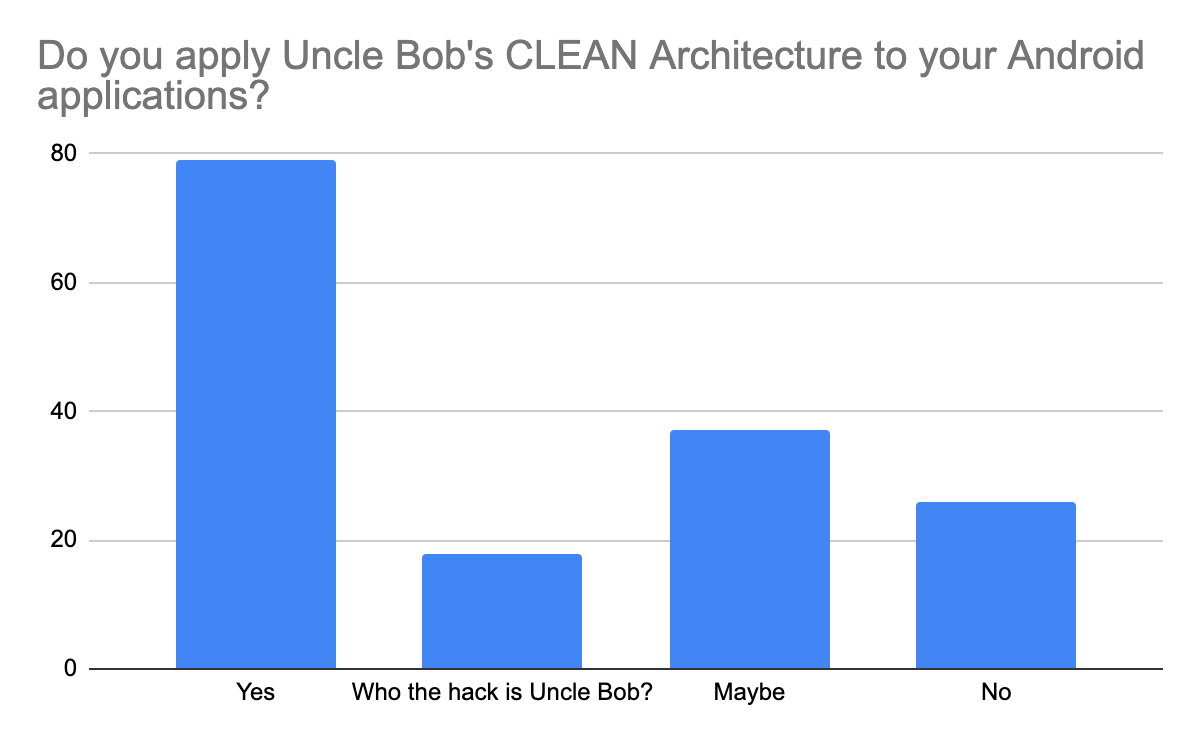
\includegraphics[scale=0.33]{figures/clean_arch.png}
    \caption{Clean Architecture usage results}
    \label{fig:clean_arch}
\end{figure}
\FloatBarrier

When examining the participatory tendencies to use Clean Architecture, it is seen that the majority of the participants adopt this architectural approach. The number of respondents who declared their use of this architectural pattern is almost more than the total of those who declared that they did not or could use it. Besides, 38 of 51 Android developers with five or more years of experience who participated in the survey declared that they use or can use this architectural pattern.

\subsubsection{Principles}
The fifth question of the survey asked the participants whether they follow SOLID principles while developing Android applications. Results have shown that 66.3\% of the participants declared that they follow SOLID principles and 20.6\% of them declared that they might follow these principles. 6.3\% of the participants stated that they do not apply the SOLID principles, and 6.9\% stated that they are not aware of these principles. The figure below contains the graphical breakdown of this data.
\begin{figure}[ht!]
    \centering
    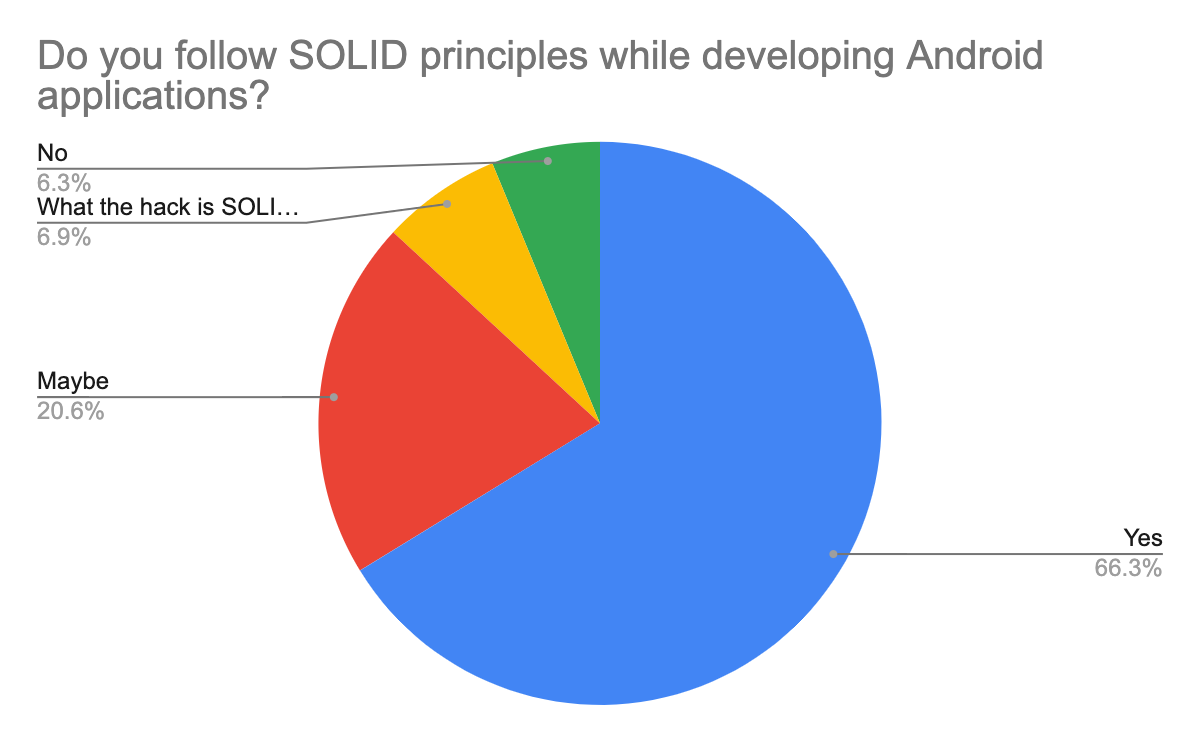
\includegraphics[scale=0.27]{figures/solid.png}
    \caption{SOLID principles usage results}
    \label{fig:solid}
\end{figure}
\FloatBarrier

The 6th question of the survey asks the participants whether they apply the "Clean Code" principles while developing Android applications. The results in the form of a pie chart can be seen below in Fig. \ref{fig:clean_code}.
\begin{figure}[ht!]
    \centering
    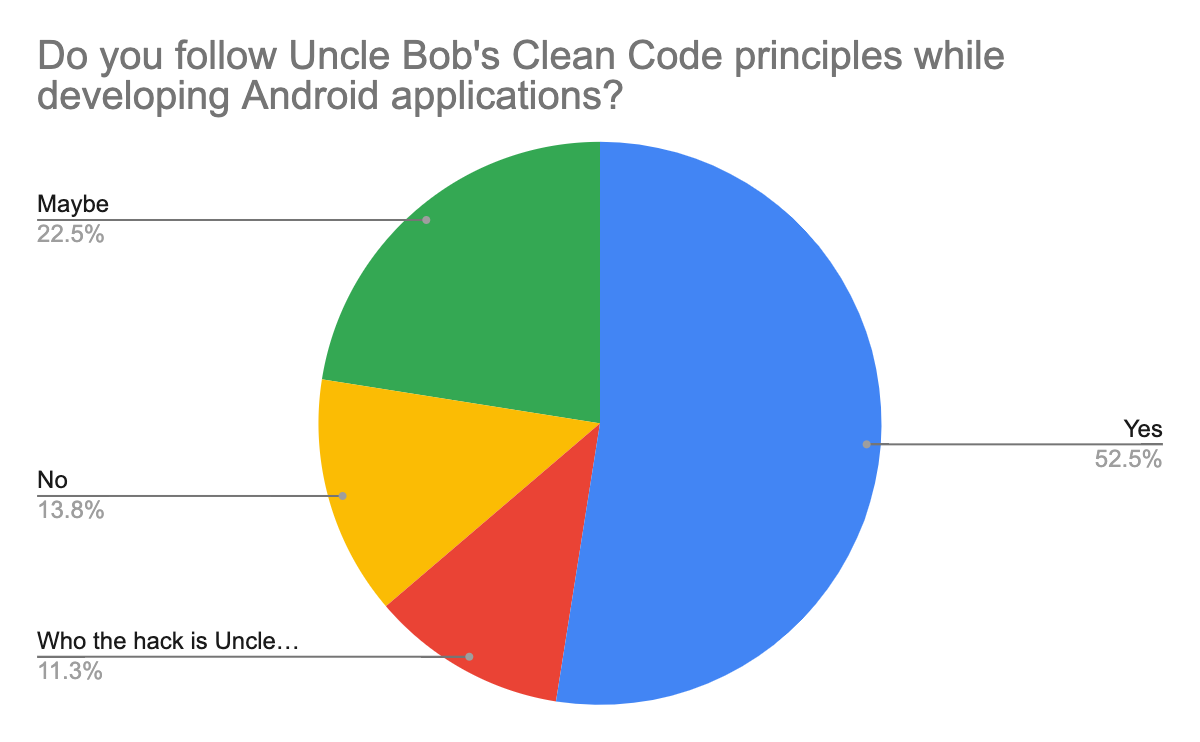
\includegraphics[scale=0.27]{figures/clean_code.png}
    \caption{Clean Code principles usage results.}
    \label{fig:clean_code}
\end{figure}
\FloatBarrier

According to the results, 75\% of the participants stated that they either used or could use these principles. While 13.8\% of the participants stated that they do not use these principles, it was observed that 11.3\% of the participants were not even aware of these principles.


\subsubsection{Libraries}
The next question is designed to ask the participants which networking library they use. Although the network library's use does not directly affect maintainability, this question was included in the questionnaire. It was also among the aims of this study to identify developer tendencies. Also, the use of some advanced networking libraries indirectly affects maintainability due to the out of box solutions they offer. For this reason, it was deemed appropriate to add this question to the survey. When looking at the answers, it is seen that the Retrofit / OkHttp library is dominating. It is observed that 75.6\% of the participants use only this library and approximately 13.8\% prefer Retrofit/OkHttp libraries and other libraries. The graphical breakdown of responses is presented below in Fig. \ref{fig:networking_lib}. It would not be wrong to say that this library is mainly preferred due to its ease when integrating back-end systems running on REST architecture into Android applications. Besides, it is seen that 9.4\% (the second-highest rate) of the participants stated that they also used the Apollo library. Apollo, which is the most efficient library used in the integration of GraphQL based back-end systems to Android applications, has the second-highest rate among the answers.
\begin{figure}[ht!]
    \centering
    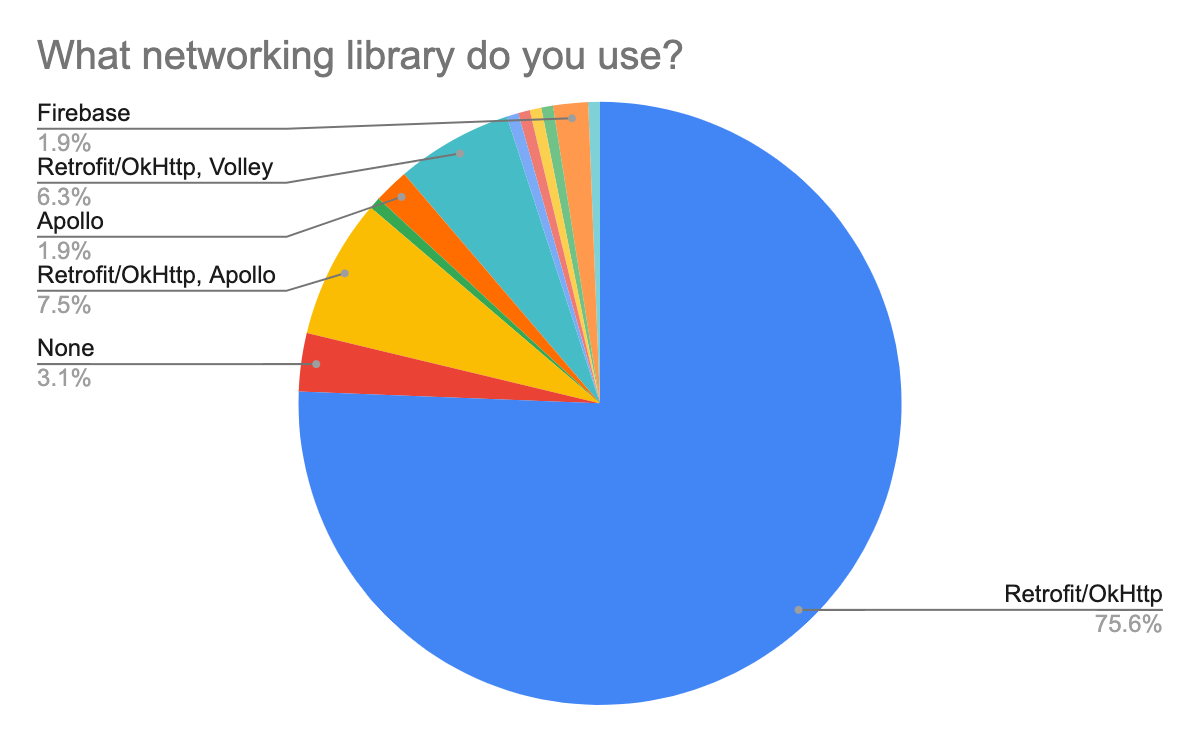
\includegraphics[scale=0.25]{figures/networking_lib.png}
    \caption{Networking library preferences results}
    \label{fig:networking_lib}
\end{figure}
\FloatBarrier

More detailed information and comments about these libraries can be found in \ref{section:4.5.2}. Mooncascade's Android team prefers Retrofit or Apollo libraries depending on the back-end system’s type to be used in the project. This preference is in line with the survey results.

The 8th question of the survey asks the question of what libraries they use to manage asynchronous processes while developing Android applications to the participants. This question was included in the survey, considering that many Android applications are based on asynchronous events and the impact of the tools used in managing these events on the application architecture and thus on maintainability. When the results are examined, it is seen that Android developers prefer the Kotlin Coroutines, RxJava and AsyncTask solutions. It is also seen that some of the participants declared that they used more than one solution. The use of more than one solution can be explained by applications that need to be maintained or preferring a solution based on the project needs. Recently, the AsyncTask solution has been deprecated by the Android team. However, it seems that some of the participants continued to use this solution. This situation can be explained by maintaining some previously coded applications using the AsyncTask and are still in use. The use of this solution is no longer recommended \cite{30}. Details of the results can be seen in the below in Fig.\ref{fig:async_events},
\begin{figure}[ht!]
    \centering
    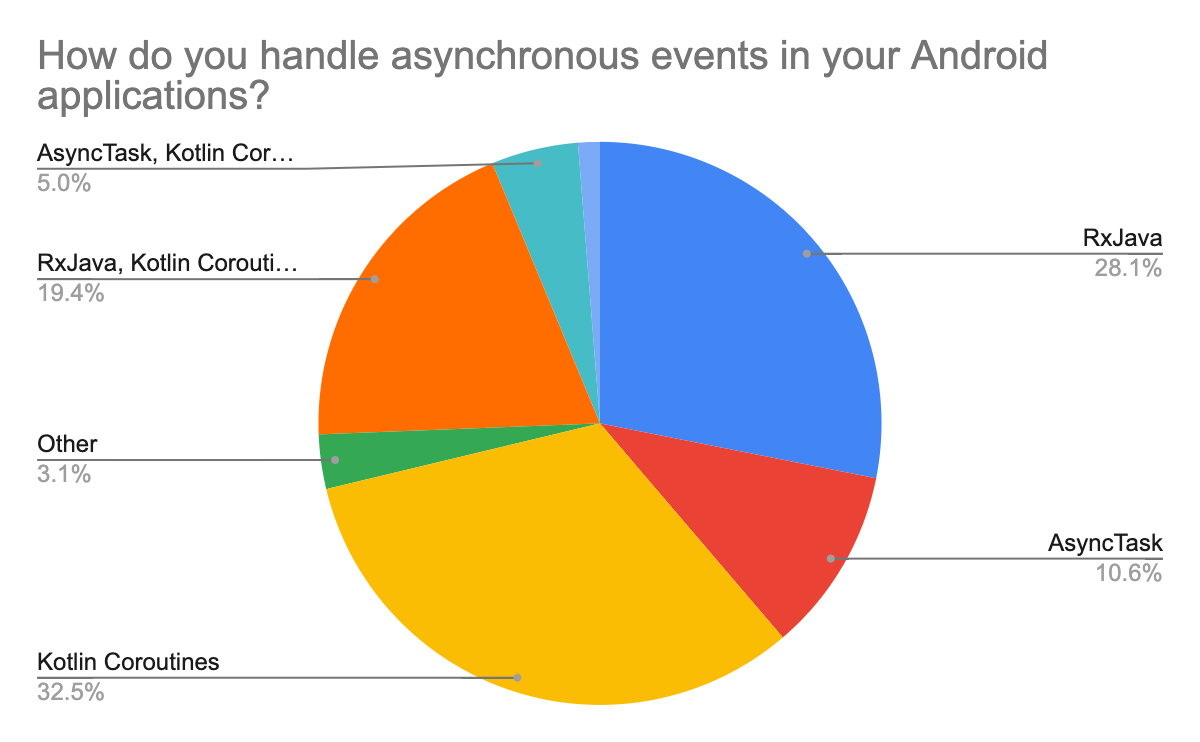
\includegraphics[scale=0.25]{figures/async_events.png}
    \caption{Threading management library preferences results}
    \label{fig:async_events}
\end{figure}
\FloatBarrier

On the other hand, we see that the Kotlin coroutines solution, which Android officially recommends \cite{31}, has the highest percentage in the survey. This solution is increasing among Android developers, as it is easier to learn and use than the RxJava library and because it requires no external dependency. Although RxJava has a steep learning curve and faces the growing popularity of the Kotlin coroutines, it is still preferred by many Android developers for the advanced features it offers. However, there has been a severe increase of applications that have recently migrated their RxJava solutions to Kotlin coroutines\cite{42}. Although the Mooncascade Android prefers RxJava for now, it has been continuing its efforts to switch to Kotlin Coroutines solution. Details on how RxJava is by used are shared in section \ref{section:4.5.3}.

The 9th question of the questionnaire asks the participants which solutions are preferred to apply dependency injection (DI) principles, which significantly impact software maintainability and software architecture when developing Android applications. As shown in Fig. \ref{fig:di_lib}, Dagger 2 is the most commonly used DI framework amongst the participant Android developers. Approximately 67.5\% of users declared that they used this solution in some way. Besides, Hilt, another DI framework developed based on Dagger 2 by Google's Android team, a relatively new technology, was able to find a place in the survey. Dagger 2 and Hilt are DI frameworks recommended by the Android team. However, it is predicted that Hilt's use will surpass Dagger 2, primarily due to the ease of learning it brings and the decrease in boilerplate code soon \cite{32}. Apart from these solutions, the Koin DI framework also stands out among the results. It can be said that the Koin is preferred among Android developers because of its ease of learning and its ability to get integrated into Android applications with much less boilerplate code when compared to Dagger 2. Also, it is essential to mention that Koin was developed by using Kotlin programming language. Finally, it is seen that 3.1\% of the participants are not aware of the concept of DI and 17.5\% of them declared that they do not use any framework for DI. This situation is not surprising given that all of the participants, who were not aware of the concept of DI, had less than a year of experience. Because DI is an advanced software development concept, and its practical implementation is a technique that requires solid experience. It is not mandatory to use any DI framework when developing Android applications. Therefore, it can be mentioned that 17.5\% of the participants stated that they do not use any framework and apply their custom solutions. Detailed results can be seen in Fig. \ref{fig:di_lib} below.
\begin{figure}[ht!]
    \centering
    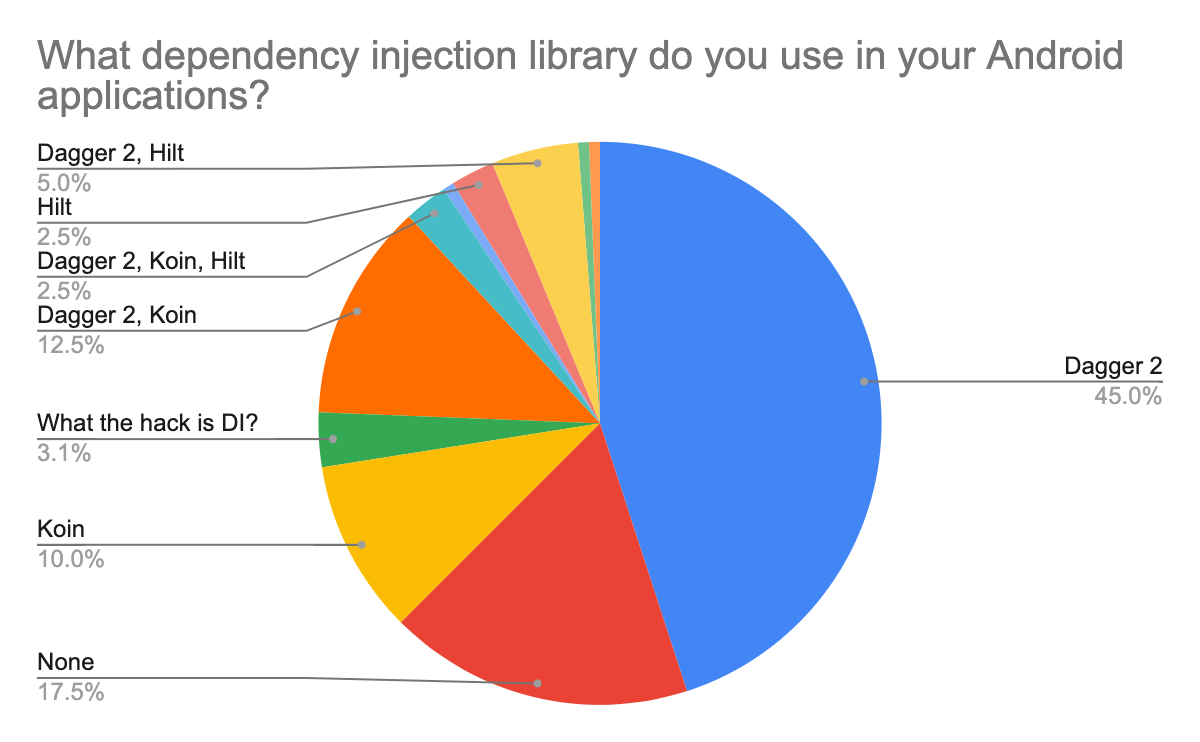
\includegraphics[scale=0.25]{figures/di_lib.png}
    \caption{DI Library preferences results}
    \label{fig:di_lib}
\end{figure}
\FloatBarrier

Mooncascade's Android team applies DI principles in their projects and makes these applications through the Dagger 2 framework. Details on how this framework is used are shared in section \ref{section:4.5.1}. The Team is also considering migrating to Hilt soon.

The final question of the survey asks respondents whether they are using the Android Architecture Components framework. When the results are examined, it is seen that more than 92\% of the participants stated that they use or can use this framework while only 7.5\% of the applicants declared that they do not use it. The high rate of usage is understandable, considering the out of box solutions it offers in solving some of the difficulties encountered while developing Android applications (which were mentioned in the first section, e.g. activity/fragment life-cycle) and the other facilities it provides for Android developers. In addition to this situation, there are groups in the Android community that are distant from this framework because it causes some other difficulties while solving the previously mentioned problems. This claim is controversial, and its details are beyond the focus of this study. However, this may be the reason why some participants do not prefer using this framework. Fig. \ref{fig:arch_components} presents the participant responses to this question in the form of a column chart.
\begin{figure}[ht!]
    \centering
    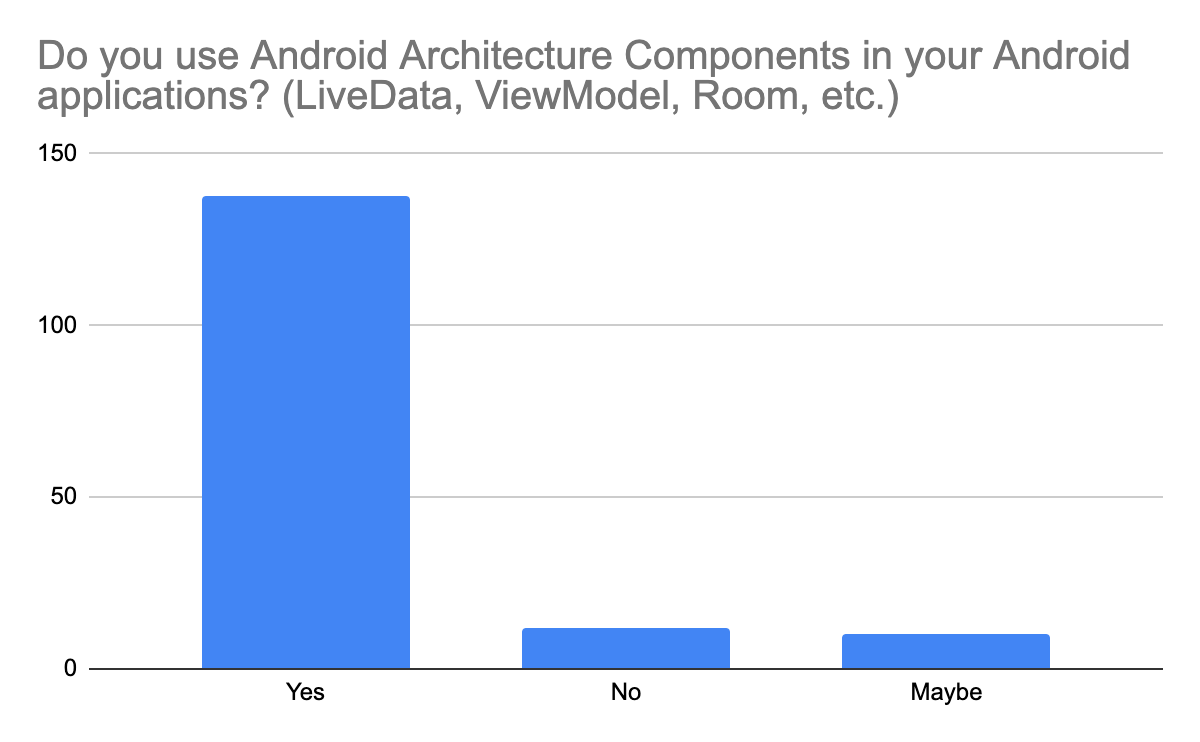
\includegraphics[scale=0.25]{figures/arch_components.png}
    \caption{Android Architecture Components usage results}
    \label{fig:arch_components}
\end{figure}
\FloatBarrier

 Mooncascade's Android team prefers to use the Android Architecture Components framework. Details on how this framework is used are shared in section \ref{section:4.5.4}.

\subsection{Interview Results}
First of all, when the results obtained from the Android developer survey are compared with the methods used by the Mooncasacade Android team, it is seen that the methods used largely overlap with the community choices. Although there are slight differences between the methods used by the team and the general Android developer choices, it can be said that these differences can be met normally. Although all the participants are Android developers, the users participating in the survey work in different companies and different domain, and it would not be wrong to say that the needs of these participants may vary according to the company and field they work in and that the methods and technologies they use are shaped according to their needs. On the other hand, the case of different user tendencies seen in the answers of the survey questions on the architectural pattern choice and the asynchronous event management libraries might be interpreted as the case company needs to re-evaluate the solutions used for these areas.Lastly, in the participants' responses to some questions, it is noteworthy that some participants choose more according to the industry trends, and this situation is observed especially in the answers given by relatively less experienced developers. As stated in the previous chapters, the Android platform is a rapidly developing platform. Therefore, it is worth noting that while choosing the methods and technologies used for developing Android applications, decisions should be made based on long-term stability and maintainability rather than industrial trends.

When the results of the interviews with the case company's Android team are examined, it is seen that the team consists of highly experienced Android developers, and they are aware of the importance of maintainability in software engineering and Android applications. Therefore, it would not be wrong to mention that the quality of the answers given by the team members to the questions in the interviews is high. First of all, five out of seven participants stated that maintainability is vital for the company and Android applications due to the way the company operates and the nature of Android applications. The other two participants stated that maintainability is already essential for software systems. These results support the theory claimed in the problem statement section of this study on maintainability that it is a critical non-functional requirement for software systems, Android applications and the case company. Besides, while the participants' evaluations about the methods and technologies used by the company in developing Android applications are generally positive, some constructive criticism also draws attention. The necessity of reconsidering the choice of architectural pattern and the asynchronous event management libraries, which was also mentioned in the Android developer survey interpretations above, was also emphasized by some case company members in the interviews. This situation stands out as a topic that the case company should focus on. The difficulties of using the RxJava library and its beginning to become out of date and the usage of Clean Architecture causing too much complexity for small and medium-sized projects are indicated as the reasons for this situation by the participants. In addition, the participants expressed their views that making the methods used into more standard coding conventions and arranging these conventions as if they were a familiar language among all members of the team would have a positive effect in terms of maintainability. Lastly, the views and awareness of most of the participants about choosing the libraries used in Android projects among stable and long-lasting libraries prove the effect of third party library use on the maintainability of Android applications.

Considering the quantitative evaluation results, some issues from CB-1 stand out. The first thing that catches the eye is a complex and unorganized packaging structure. Layer and feature-based packaging methods are internal in the project, which cause serious maintainability, understandability and organization problems. It is also noteworthy that some classes are large in size, which can be interpreted as lack of proper separation of concerns. The codebase appears to have complexity, coupling and cohesion problems as well. In a few classes, these problems are at a very high level, and maintainability and organization problems at different levels in the project draw attention. Especially the coupling problem stands out for this code base. Considering that there are no healthy abstraction and dependency injection application in the project, this result is not very surprising. When all these analysis results are taken into account, it is clear that the cb-1 codebase shows a low maintainability character. Nevertheless, cb-1's situation offered an opportunity for this study to evaluate maintainability. On the other hand, results of CB-2 has shown that there are visible improvements in complexity, coupling and cohesion. In addition, significantly reduced entity sizes and increased class and package numbers were noticed. Concise classes and the increase in the number of packages point to a more organized code base and a better separation of concerns, making the understandability of the codebase high. Besides, the levels of the classes in complexity, coupling are quite low, and cohesion is high. This situation can be shown as proof that the SOLID and SoC principles are applied correctly, and it can be said that there is a very positive effect on maintainability. However, a few classes with moderate complexity and cohesion issues stand out. When these classes were investigated, it was seen that they were the classes called "View Model" in the MVVM design pattern that are responsible for how and when the data will be displayed. According to the principles of the MVVM design pattern, each view should have only one view model. In this case, the view models belonging to the views with more than one responsibility also have the logic of belonging to more than one responsibility. Therefore, these classes become more complex, and the cohesion of the classes decreases due to the methods and dependencies they have for different responsibilities. As long as the principles of the MVVM design pattern are followed, it would not be appropriate to divide these responsibilities between different classes. Nevertheless, the effects of the technology and principles used in the development of cb-2 on maintainability are obvious.

When the feature-based comparison results between the two codebases are examined, it is seen that the cb-1 codebase uses 6 classes and interfaces for the visual part of the login feature, while cb-2 uses only 2 classes for this feature. From this point of view, the cb-2 code is better in terms of organization and understandability. Also, the metric values presented in Fig. \ref{fig:login-metric-table} have shown that the results of cb-2 are better than the results of cb-1. In addition, the metric values presented in Fig. \ref{fig:login-metric-table-2} has shown the difference between the view responsibilities of the two projects on complexity. When the values of WMC, DIT and NOC metrics used in complexity measurement are compared, it is seen that the complexity level of cb-2 for the view responsibility is lower. On the other hand, when the results of the complexity metric values of view logic related responsibilities are examined, it is observed that there is not much difference between the two code bases. As explained in previous sections, these results should be considered normal given the complexity of functionality of the classes involved in this responsibility. When the CBO metric related to measuring the coupling level is examined, it is seen that the cb-2 codebase gives better results. Since the SOLID and DI principles are used much more effectively in the cb-2 codebase, these results are not different from what is expected. Also, cb-1 uses the MVP design pattern. Coupling is increasing due to the bi-directional dependency between view and presentation layers in the MVP design pattern. It would not be wrong to say that this situation increases the coupling level of the cb-1. However, this situation is not the case for cb-2, which uses the MVVM design pattern. In the MVVM design pattern, only the view layer has a dependency to the presentation layer. When the results of the LCOM metric related to cohesion are examined, it is seen that the results are similar to the results of the complexity metrics. While the results of cb-2 are much better than cb-1 for the responsibility of view, there is not much difference between the results for the responsibility of presentation. As explained in the previous section, there is only one view model per view principle in the MVVM design pattern. Therefore, one view model might have different responsibilities, especially those that belong to the complex views. The same is true for the MVP design pattern as well. There can be only one presenter for each view. Naturally, cb-1, which uses the MVP design pattern, seems to have low cohesion values for presentation responsibility. Ultimately, results obtained from the qualitative and quantitative evaluations have shown that the effects of the methods and technologies used by the case company on the maintainability of Android applications are seen as positive, yet some points need improvement. The results also showed the importance of maintainability for the software systems, Android applications and particularly for the case company. 

\subsection{Quantitative Evaluation Results}
Within the scope of this study, qualitative and quantitative methods to evaluate the methods and technologies used by Mooncascade's Android team were conducted. There were some limitations during the process these evaluations. 
First of all, it should be stated that the features used in quantitative evaluations are relatively less complex features of the Android application used for the evaluation. Therefore the efficiency of evaluation and comparison was affected by this situation. Using more complex feature could provide better insight into the impact of the methods and technologies used by the case company. Unfortunately, this was not possible within the scope of this study due to a lack of features and time to develop more complex features. However, it is true that using relatively less complicated features while making the assessment slightly reduces the results' effectiveness. Still, it does not mean that these results are false or unrealistic. Also, considering that there may be deficiencies in the methods used in the evaluations, the necessity to carry out more detailed studies on how to evaluate maintainability better and how to develop Android applications in terms of maintainability is obvious For example, there are different methods to evaluate the software system's maintainability, and different metrics can be used. Therefore choosing the most efficient metrics to measure the maintainability of software systems and Android applications is controversial. Further research should be conducted to find the most efficient quantitative evaluation method. In addition, this study provides an overview rather than measuring the impact of each technology and method used by the case company to maintainability individually. The study does not provide detailed information on how much effect which matter has on maintainability. From this point of view, this can be seen as a limitation for this study. Lastly, although very important information was collected within the scope of qualitative evaluations, the number of participants is relatively low. More accurate and more reflective results can be obtained with interviews and surveys with a higher number of participants.

\subsection{Summary}
In this section, details of the qualitative and quantitative evaluation methods performed within the scope of this study and the results of these evaluations are shared. The qualitative methods are the Android developer questionnaire and interviews with the Mooncascade Android team. In contrast, the quantitative method consists of the measurements of five metrics applied with the CodeMR static code analysis tool. The interpretation of these evaluations, the results of which are shared in this section, will be carried out in the next section.

\newpage
\section{Discussion}
\label{section:6}
\subsection{RQ1 Discussion}
First of all, the information obtained while answering the first research question guided the whole of this study. Research conducted to answer RQ1 has shown that the use of quantitative measurements together with qualitative measures can increase the effectiveness of the study. It was seen that qualitative measurements can make important contributions to the results of the evaluation with the information obtained directly from the developers and support the quantitative measurement results. The fact that experienced Android developers make evaluations about the methods and technologies they use every day from the maintainability point of view and the results obtained from these evaluations can be added to this study increased the study's accuracy. From this point of view, it would not be wrong to say that the addition of qualitative methods as well as quantitative methods to studies focusing on the measurement of software development concepts such as maintainability would increase the qualification of the study. The research conducted to answer the first research question showed that the maintainability of object-oriented software systems can be evaluated quantitatively by using many different metrics. In this study, a different quantitative maintainability model based on the concepts of complexity, coupling and cohesion was formed to measure the maintainability of Android applications. This model was created by inspiring the problems encountered while developing Android applications, mentioned in section \ref{section:1.1}. Subsequently, 5 metrics that are suitable for this evaluation model and can measure these concepts were determined. However, it cannot be said that these methods and metrics used in this study is the best that can be used for this purpose. Although these methods and metrics were sufficient for this study, it would not be wrong to say that there may be more effective quantitative measurement methods. It would be appropriate to conduct comparative studies to determine the most effective solution. 

\subsection{RQ2 Discussion}
First of all, when the results obtained from the Android developer survey are compared with the methods used by the Mooncasacade Android team, it is seen that the methods used largely overlap with the community choices. There are slight differences (e.g. the preference of Kotlin Coroutines in the Android community, different design patterns) between the methods used by the team and the Android developer tendencies, but it can be said that these differences can be met normally. Although all the participants are Android developers, the users participating in the survey work in different companies and different domain, and it would not be wrong to say that the needs of these participants may vary according to the company and field they work in and that the methods and technologies they use are shaped according to their needs. On the other hand, the case of different user tendencies seen in the answers of the survey questions on the architectural pattern choice and the asynchronous event management libraries might be interpreted as the case company needs to re-evaluate the solutions used for these areas.Lastly, in several participants' responses, it was noticed that they choose based on the industry trends, and this situation is observed especially in the answers given by relatively less experienced developers. As stated in the previous chapters, the Android platform is a rapidly developing platform. Therefore, it is worth noting that while choosing the methods and technologies used for developing Android applications, decisions should be made based on long-term stability and maintainability rather than industrial trends.

When the results of the interviews with the case company's Android team were examined, it was seen that the team consists of highly experienced Android developers, and they are aware of the importance of maintainability in software engineering and Android applications. Therefore, it would not be wrong to mention that the quality of the answers given by the team members to the questions in the interviews is high. First of all, five out of seven participants stated that maintainability is vital for the company and Android applications due to the way the company operates and the nature of Android applications. The other two participants stated that maintainability is already essential for software systems. These results support the theory claimed in the problem statement section of this study that maintainability is a critical non-functional requirement for software systems, Android applications and the case company. Besides, while the participants' evaluations about the methods and technologies used by the company in developing Android applications are generally positive, some constructive criticism also draws attention. The necessity of reconsidering the choice of architectural pattern and the asynchronous event management libraries, which was also mentioned in the Android developer survey interpretations above, was also emphasized by some case company members in the interviews. This situation stands out as a topic that the case company should focus on. The difficulties of using the RxJava library and its beginning to become out of date and the usage of Clean Architecture causing too much complexity for small and medium-sized projects are indicated as the reasons for this situation by the participants. In addition, the participants expressed their views that making the methods used into more standard coding conventions and arranging these conventions as if they were a familiar language among all members of the team would have a positive effect in terms of maintainability. Lastly, the views and awareness of most of the participants about choosing the libraries used in Android projects among stable and long-lasting libraries prove the effect of third party library use on the maintainability of Android applications.

Considering the quantitative evaluation results, some issues from CB-1 stand out. The first thing that catches the eye is a complex and unorganized packaging structure. Layer and feature-based packaging methods are internal in the project, which cause serious maintainability, understandability and organization problems. It is also noteworthy that some classes are large in size, which can be interpreted as lack of proper separation of concerns. The codebase appears to have complexity, coupling and cohesion problems as well. In a few classes, these problems are at a very high level, and maintainability and organization problems at different levels in the project draw attention. Especially the high coupling problem stands out for this code base. Considering that there are no healthy abstraction and dependency injection application in the project, this result is not very surprising. When all these analysis results are taken into account, it is clear that the CB-1 codebase shows a low maintainability character. Nevertheless, CB-1's situation offered an opportunity for this study to evaluate maintainability. On the other hand, results of CB-2 has shown that there are visible improvements in complexity, coupling and cohesion. In addition, significantly reduced entity sizes and increased class and package numbers were noticed. Concise classes and the increase in the number of packages point to a more organized code base and a better separation of concerns, making the understandability of the codebase high. Besides, the levels of the classes in complexity, coupling are quite low, and cohesion is high. This situation can be shown as proof that the SOLID and SoC principles are applied correctly, and it can be said that there is a very positive effect on maintainability. However, a few classes with moderate complexity and cohesion issues stand out. When these classes were investigated, it was seen that they were the classes called "View Model" in the MVVM design pattern that are responsible for how and when the data will be displayed. According to the principles of the MVVM design pattern, each view should have only one view model. In this case, the view models belonging to the views with more than one responsibility also have the logic of belonging to more than one responsibility. Therefore, these classes become more complex, and the cohesion of the classes decreases due to the methods and dependencies they have for different responsibilities. As long as the principles of the MVVM design pattern are followed, it would not be appropriate to divide these responsibilities between different classes. Nevertheless, the positive effects of the technology and principles used in the development of CB-2 on maintainability are obvious.

\subsection{RQ3 Discussion}
First of all, it should be stated that the features used in quantitative evaluations were relatively less complex features of the Android application. Therefore the efficiency of evaluation and comparison was affected by this situation. Using more complex features could have provided better insight into the impact of the methods and technologies used by the case company. Unfortunately, this was not possible within the scope of this study due to not having the time required to develop more complex features. Still, it does not mean that these results are false or unrealistic. Moreover, considering that there may be insufficiencies in the methods used in the evaluations, the necessity to carry out more detailed studies to find a proper method for evaluating the maintainability of Android applications is undeniable. For example, there are different methods to evaluate the software system's maintainability, and different metrics can be used. Therefore choosing the most efficient metrics to measure the maintainability of software systems and Android applications is controversial, especially when the differences of Android applications are taken into account. Further research should be conducted to find the most efficient quantitative evaluation method.

\subsection{Limitations}
\input{chapters/6-discussion/6.4-limitations/6.4-text}

\clearpage
\section{Conclusion}
\label{section:7}
This study covered the subject of evaluating the impact of the methods and technologies used by the software product development company Mooncascade while developing Android applications on the maintainability of these applications.
There are four major challenges encountered when developing Android applications. These challenges are Android’s nature, demanding business needs, the frequent update rate of Android applications, and changing development teams. A maintainability model was formed by focusing on these major challenges. This model was formed based on the correlation between the major Android development challenges and the well-known software engineering concepts such as complexity, coupling and cohesion, whose relationships with maintainability were proven. While applying this maintainability model, quantitative and qualitative evaluation methods have been used. Quantitative and qualitative evaluation methods were determined to measure maintainability and the evaluations were carried out using these methods. To make a qualitative evaluation, a public Android survey was carried out with random Android developers and interviews were conducted with each member of the Android team of the company. To make the quantitative evaluation, a set of object-oriented software metrics were used. These metrics were applied to common features of the different codebases belonging to the same project through the CodeMR static code analysis tool.

First of all, this study has demonstrated the importance of maintainability for Android applications and addressed the important matters in terms of the maintainability of Android applications. These matters stand out as usage of principles and conventions to increase software understandability, implementing human-readable code, proper software architecture and design pattern selection and use of stable third-party libraries. Quantitative and qualitative evaluations proved that the maintainability of Android applications developed by paying attention to these matters will increase. Moreover, results indicated the positive impact of the methods and technologies used by the case company on the maintainability of Android applications. The comparison between the two codebases, one developed using the case company's methods and technologies, the other developed without a specific order and standard, showed that even for the relatively simple application features, maintainability had been increased. Outcomes also revealed the shortcomings and areas open to improvement for the methods and technologies used by the case company. The areas open to improvement are re-evaluating the use of libraries that are in danger of becoming outdated, such as RxJava, architectural scaling and selection according to the project, and making the coding conventions more standardized. It is predicted that re-evaluating these issues will further increase the positive effect on the maintainability of Android applications. 

Lastly, the findings obtained as a result of answering the first research question showed that a new model is needed to measure the maintainability of Android applications. The main reason for this need is the differences of Android applications from traditional software systems and their update rates. Especially Android's unique ecosystem points out the need for new methods and metrics to measure the maintainability of applications running on this ecosystem. While creating these new metrics, it is anticipated that besides the specific dynamics of Android applications, it may also be beneficial to use metrics that can include effort and time measurement that can be associated with high updating rates of the Android applications.

\subsection{Future Work}
Considering the lack of methods that can effectively measure the maintainability of Android applications, it would not be wrong to say that future research will focus on this issue as a continuation of this study. In addition, in the case of determining these methods, it is also among the targets to try the methods on more complex application features and get more effective results, thus eliminating the limitations of this study.

\newpage
\printbibliography
\addcontentsline{toc}{section}{References}

\newpage
\section*{Appendix}
\addcontentsline{toc}{section}{Appendix}
%\section*{I. Glossary}
%\addcontentsline{toc}{subsection}{I. Glossary}
%\TODO{What to do here?}
%\newpage

%=== Licence in English
\newcommand{\licencehint}[2]{\\\hspace*{#1}\textsl(#2)\par}
\newcommand\EngLicence{{%
\selectlanguage{english}
\section*{I. Licence}

\addcontentsline{toc}{subsection}{II. Licence}

\subsection*{Non-exclusive licence to reproduce thesis and make thesis public}
I, \textbf{Mustafa Ogün Öztürk}, %author's name

\begin{enumerate}
\item
herewith grant the University of Tartu a free permit (non-exclusive licence) to
\par
reproduce, for the purpose of preservation, including for adding to the DSpace digital archives until the expiry of the term of copyright,
\par
\textbf{Evaluating Maintainability of Android Applications: Mooncascade Case Study}, %

\par
supervised by Jakob Mass. %supervisor's name
  
\item
I grant the University of Tartu a permit to make the work specified in p. 1 available to the public via the web environment of the University of Tartu, including via the DSpace digital archives, under the Creative Commons licence CC BY NC ND 3.0, which allows, by giving appropriate credit to the author, to reproduce, distribute the work and communicate it to the public, and prohibits the creation of derivative works and any commercial use of the work until the expiry of the term of copyright.
\item
I am aware of the fact that the author retains the rights specified in p. 1 and 2.
\item
I certify that granting the non-exclusive licence does not infringe other persons' intellectual property rights or rights arising from the personal data protection legislation. 
\end{enumerate}

\noindent
Mustafa Ogün Öztürk\\ %author's name
\textbf{\textsl{14/05/2021}}
}}%\newcommand\EngLicence

%=== Licence in Estonian
\newcommand\EstLicence{{%
\selectlanguage{estonian}
\section*{II. Litsents}

\addcontentsline{toc}{subsection}{II. Litsents}

\subsection*{Lihtlitsents lõputöö reprodutseerimiseks ja üldsusele kättesaadavaks tegemiseks}

Mina, \textbf{Alice Cooper}, %author's name
  \licencehint{10mm}{autori nimi}

\begin{enumerate}
\item
annan Tartu Ülikoolile tasuta loa (lihtlitsentsi) minu loodud teose
\par
\textbf{Tüübituletus neljandat järku loogikavalemitele}, %title of thesis
    \licencehint{10mm}{lõputöö pealkiri}
\par
mille juhendaja(d) on Axel Rose ja May Flower, %supervisor's name(s)
  \licencehint{10mm}{juhendaja nimi}
\par
reprodutseerimiseks eesmärgiga seda säilitada, sealhulgas lisada digitaalarhiivi DSpace kuni autoriõiguse kehtivuse lõppemiseni.
\par
\item
Annan Tartu Ülikoolile loa teha punktis 1 nimetatud teos üldsusele kättesaadavaks Tartu Ülikooli veebikeskkonna, sealhulgas digitaalarhiivi DSpace kaudu Creative Commonsi litsentsiga CC BY NC ND 3.0, mis lubab autorile viidates teost reprodutseerida, levitada ja üldsusele suunata ning keelab luua tuletatud teost ja kasutada teost ärieesmärgil, kuni autoriõiguse kehtivuse lõppemiseni.
\item
Olen teadlik, et punktides 1 ja 2 nimetatud õigused jäävad alles ka autorile.
\item
Kinnitan, et lihtlitsentsi andmisega ei riku ma teiste isikute intellektuaalomandi ega isikuandmete kaitse õigusaktidest tulenevaid õigusi. 
\end{enumerate}

\noindent
Alice Cooper\\ %author's name
\textbf{\textsl{pp.kk.aaaa}}
}}%\newcommand\EstLicence


%===Choose the licence in active language
\iflanguage{english}{\EngLicence}{\EstLicence}

\end{document}